% -------------------------------------------------------------------------
% ------ nuweb macros (redefine as desired, or omit with "nuweb -p") ------
% -------------------------------------------------------------------------
\providecommand{\NWtxtMacroDefBy}{Macro defined by}
\providecommand{\NWtxtMacroRefIn}{Macro referenced in}
\providecommand{\NWtxtMacroNoRef}{Macro never referenced}
\providecommand{\NWtxtDefBy}{Defined by}
\providecommand{\NWtxtRefIn}{Referenced in}
\providecommand{\NWtxtNoRef}{Not referenced}
\providecommand{\NWtxtFileDefBy}{File defined by}
\providecommand{\NWsep}{${\diamond}$}
\providecommand{\NWlink}[2]{\hyperlink{#1}{#2}}
\providecommand{\NWtarget}[2]{% move baseline up by \baselineskip 
  \raisebox{\baselineskip}[1.5ex][0ex]{%
    \mbox{%
      \hypertarget{#1}{%
        \raisebox{-1\baselineskip}[0ex][0ex]{%
          \mbox{#2}%
}}}}}
% -------------------------------------------------------------------------

\documentclass[11pt,oneside]{article}	%use"amsart"insteadof"article"forAMSLaTeXformat
\usepackage{geometry}		%Seegeometry.pdftolearnthelayoutoptions.Therearelots.
\geometry{letterpaper}		%...ora4paperora5paperor...
%\geometry{landscape}		%Activateforforrotatedpagegeometry
%\usepackage[parfill]{parskip}		%Activatetobeginparagraphswithanemptylineratherthananindent
\usepackage{graphicx}				%Usepdf,png,jpg,oreps•withpdflatex;useepsinDVImode
								%TeXwillautomaticallyconverteps-->pdfinpdflatex		
\usepackage{amssymb}
\usepackage{hyperref}

%----macros begin---------------------------------------------------------------
\usepackage{color}
\usepackage{amsthm}

\def\conv{\mbox{\textrm{conv}\,}}
\def\aff{\mbox{\textrm{aff}\,}}
\def\E{\mathbb{E}}
\def\R{\mathbb{R}}
\def\Z{\mathbb{Z}}
\def\tex{\TeX}
\def\latex{\LaTeX}
\def\v#1{{\bf #1}}
\def\p#1{{\bf #1}}
\def\T#1{{\bf #1}}

\def\vet#1{{\left(\begin{array}{cccccccccccccccccccc}#1\end{array}\right)}}
\def\mat#1{{\left(\begin{array}{cccccccccccccccccccc}#1\end{array}\right)}}

\def\lin{\mbox{\rm lin}\,}
\def\aff{\mbox{\rm aff}\,}
\def\pos{\mbox{\rm pos}\,}
\def\cone{\mbox{\rm cone}\,}
\def\conv{\mbox{\rm conv}\,}
\newcommand{\homog}[0]{\mbox{\rm homog}\,}
\newcommand{\relint}[0]{\mbox{\rm relint}\,}

%----macros end-----------------------------------------------------------------

\title{Boolean Chains: set operations with topological chains
\footnote{This document is part of the \emph{Linear Algebraic Representation with CoChains} (LAR-CC) framework~\cite{cclar-proj:2013:00}. \today}
}
\author{Alberto Paoluzzi}
%\date{}							%Activatetodisplayagivendateornodate

\begin{document}
\maketitle
%\nonstopmode

%----macros end-----------------------------------------------------------------
%>>>>>>>>>>>>>>>>>>>>>>>>>>>>>>>>>>>>>>>>>>>>>>>>>>>>>>>>>>>>>>>>>>>>>>>>>>>>>>>
\begin{abstract}
Boolean operations are a major addition to every geometric package. Union, intersection, difference and complementation of decomposed spaces are discussed and implemented in this module by making use of the Linear Algebraic Representation (LAR) introduced in~\cite{Dicarlo:2014:TNL:2543138.2543294}. First, the two finite decompositions are merged, by merging their vertices (0-cells of support spaces); then a Delaunay complex based on the vertex set union is computed, and the shared $d$-chain is extracted and split, according to the cellular structure of the input $d$-chains. The results of a Boolean operation are finally computed by sum, product or difference of the (binary) coordinate representation of the (split) argument chains, by using the novel chain-basis resulted from the splitting step. Differently from the totality of algorithms known to the authors, neither search nor traversal of some (complicated) data structure is performed by this algorithm. 
\end{abstract}

\tableofcontents
%<<<<<<<<<<<<<<<<<<<<<<<<<<<<<<<<<<<<<<<<<<<<<<<<<<<<<<<<<<<<<<<<<<<<<<<<<<<<<<<
%>>>>>>>>>>>>>>>>>>>>>>>>>>>>>>>>>>>>>>>>>>>>>>>>>>>>>>>>>>>>>>>>>>>>>>>>>>>>>>>
\section{Introduction}

In this section we introduce and shortly outline our novel algorithm for Boolean operations with chain of cells from different space decompositions implemented in this LAR-CC software module.

The input objects are denoted in the remainder as $X_1$ and $X_2$, and their finite cell decompositions as $\Lambda^1$ and $\Lambda^1$. Our goal is to compute $X = X_1\, op\, X_2$, where $op \in \{\cup ,\cap , - ,\ominus \}$ or $\complement X$, based on a common decomposition $\Lambda = \Lambda^1\, op\, \Lambda^2$, with $\Lambda$ being a suitably fragmented decomposition of the X space.

Of course, we aim to compute a minimal (in some sense) decomposition, making the best use of the LAR framework, based on CSR representation of sparse binary matrices and standard matrix algebra operations.
However, in this first implementation of the chain approach to Boolean operations, we are satisfied with a solution using simplicial triangulations of input spaces. Future revisions of our algorithm will be based on more general cellular complexes.

\subsection{User interface}

The API will contain the high-level binary functions \texttt{union}, \texttt{intersection}, \texttt{difference}, and \texttt{xor}. Each of them will call the same function \texttt{boolOps} and then suitably operates the two returned bit arrays, i.e.~the coordinate representations of the input spaces in the merged cell decomposition. The input parameters \texttt{lar1} and  \texttt{lar2} stand for two LAR models, each one constituted by a pair \texttt{(V,CV)}, i.e.~by the matrix \texttt{V} of vertex coordinates and by an integer array \texttt{CV} giving the vertex indices of each $d$-cell.

%-------------------------------------------------------------------------------
\begin{flushleft} \small \label{scrap1}
\protect\makebox[0ex][r]{\NWtarget{nuweb2}{\rule{0ex}{0ex}}\hspace{1em}}$\langle\,$High-level boolean operations\nobreak\ {\footnotesize 2}$\,\rangle\equiv$
\vspace{-1ex}
\begin{list}{}{} \item
\mbox{}\verb@def union(lar1,lar2):@\\
\mbox{}\verb@   lar = boolOps(lar1,lar2)@\\
\mbox{}\verb@def intersection(lar1,lar2):@\\
\mbox{}\verb@   lar = boolOps(lar1,lar2)@\\
\mbox{}\verb@def difference(lar1,lar2):@\\
\mbox{}\verb@   lar = boolOps(lar1,lar2)@\\
\mbox{}\verb@def xor(lar1,lar2):@\\
\mbox{}\verb@   lar = boolOps(lar1,lar2)@\\
\mbox{}\verb@@{\NWsep}
\end{list}
\vspace{-1ex}
\footnotesize\addtolength{\baselineskip}{-1ex}
\begin{list}{}{\setlength{\itemsep}{-\parsep}\setlength{\itemindent}{-\leftmargin}}
\item \NWtxtMacroRefIn\ \NWlink{nuweb13a}{13a}.
\end{list}
\end{flushleft}
%-------------------------------------------------------------------------------

%<<<<<<<<<<<<<<<<<<<<<<<<<<<<<<<<<<<<<<<<<<<<<<<<<<<<<<<<<<<<<<<<<<<<<<<<<<<<<<<
%>>>>>>>>>>>>>>>>>>>>>>>>>>>>>>>>>>>>>>>>>>>>>>>>>>>>>>>>>>>>>>>>>>>>>>>>>>>>>>>
\section{Merging 0-cells}
%<<<<<<<<<<<<<<<<<<<<<<<<<<<<<<<<<<<<<<<<<<<<<<<<<<<<<<<<<<<<<<<<<<<<<<<<<<<<<<<

The real work is performed by the function \texttt{boolOps}, that will procede step-by-step (see Section~\ref{sec:splitting}) to the computation of the minimally fragmented common cell complex where to compute the chain resulting from the requested Boolean operation.

%-------------------------------------------------------------------------------
\subsection{Global reordering of vertex coordinates}
%-------------------------------------------------------------------------------
A global reordering of vertex coordinates is executed as the first step of the Boolean algorithm, in order to eliminate the duplicate vertices, by substituting double vertex copies (coming from the two close points) with a single instance. 

Two dictionaries are created, then merged in a single dictionary, and finally split into three subsets of (vertex,index) pairs, with the aim of rebuilding the input representations, by making use of a novel and more useful vertex indexing.

The union set of vertices is finally reordered using the three subsets of vertices belonging (a) only to the first argument, (b) only to the second argument and (c) to both, respectively denoted as $V_1, V_2, V_{12}$. A top-down description of this initial computational step is provided by the set of macros discussed in this section.

%-------------------------------------------------------------------------------
\begin{flushleft} \small \label{scrap2}
\protect\makebox[0ex][r]{\NWtarget{nuweb3a}{\rule{0ex}{0ex}}\hspace{1em}}$\langle\,$Place the vertices of Boolean arguments in a common space\nobreak\ {\footnotesize 3a}$\,\rangle\equiv$
\vspace{-1ex}
\begin{list}{}{} \item
\mbox{}\verb@""" First step of Boolen Algorithm """@\\
\mbox{}\verb@@\hbox{$\langle\,$Initial indexing of vertex positions\nobreak\ {\footnotesize \NWlink{nuweb3b}{3b}}$\,\rangle$}\verb@@\\
\mbox{}\verb@@\hbox{$\langle\,$Merge two dictionaries with keys the point locations\nobreak\ {\footnotesize \NWlink{nuweb3c}{3c}}$\,\rangle$}\verb@@\\
\mbox{}\verb@@\hbox{$\langle\,$Filter the common dictionary into three subsets\nobreak\ {\footnotesize \NWlink{nuweb4a}{4a}}$\,\rangle$}\verb@@\\
\mbox{}\verb@@\hbox{$\langle\,$Compute an inverted index to reorder the vertices of Boolean arguments\nobreak\ {\footnotesize \NWlink{nuweb4b}{4b}}$\,\rangle$}\verb@@\\
\mbox{}\verb@@\hbox{$\langle\,$Return the single reordered pointset and the two $d$-cell arrays\nobreak\ {\footnotesize \NWlink{nuweb5a}{5a}}$\,\rangle$}\verb@@\\
\mbox{}\verb@@{\NWsep}
\end{list}
\vspace{-1ex}
\footnotesize\addtolength{\baselineskip}{-1ex}
\begin{list}{}{\setlength{\itemsep}{-\parsep}\setlength{\itemindent}{-\leftmargin}}
\item \NWtxtMacroRefIn\ \NWlink{nuweb13a}{13a}.
\end{list}
\end{flushleft}
%-------------------------------------------------------------------------------

%-------------------------------------------------------------------------------
\subsubsection{Re-indexing of vertices}
%-------------------------------------------------------------------------------

\paragraph{Initial indexing of vertex positions}
The input LAR models are located in a common space by (implicitly) joining \texttt{V1} and \texttt{V2} in a same array, and (explicitly) shifting the vertex indices in \texttt{CV2} by the length of \texttt{V1}.
%-------------------------------------------------------------------------------
\begin{flushleft} \small \label{scrap3}
\protect\makebox[0ex][r]{\NWtarget{nuweb3b}{\rule{0ex}{0ex}}\hspace{1em}}$\langle\,$Initial indexing of vertex positions\nobreak\ {\footnotesize 3b}$\,\rangle\equiv$
\vspace{-1ex}
\begin{list}{}{} \item
\mbox{}\verb@from collections import defaultdict, OrderedDict@\\
\mbox{}\verb@@\\
\mbox{}\verb@def vertexSieve(model1, model2):@\\
\mbox{}\verb@   V1,CV1 = model1; V2,CV2 = model2@\\
\mbox{}\verb@   n = len(V1); m = len(V2)@\\
\mbox{}\verb@   def shift(CV, n): @\\
\mbox{}\verb@      return [[v+n for v in cell]for cell in CV]@\\
\mbox{}\verb@   CV2 = shift(CV2,n)@\\
\mbox{}\verb@@{\NWsep}
\end{list}
\vspace{-1ex}
\footnotesize\addtolength{\baselineskip}{-1ex}
\begin{list}{}{\setlength{\itemsep}{-\parsep}\setlength{\itemindent}{-\leftmargin}}
\item \NWtxtMacroRefIn\ \NWlink{nuweb3a}{3a}.
\end{list}
\end{flushleft}
%-------------------------------------------------------------------------------

\paragraph{Merge two dictionaries with point location as keys}
Since currently \texttt{CV1} and \texttt{CV2} point to a set of vertices larger than their initial sets 
\texttt{V1} and \texttt{V2}, we index the set $\texttt{V1} \cup \texttt{V2}$ using a Python \texttt{defaultdict} dictionary, in order to avoid errors of "missing key". As dictionary keys, we use the string representation of the vertex position vector provided by the \texttt{vcode} function given in the Appendix.
%-------------------------------------------------------------------------------
\begin{flushleft} \small \label{scrap4}
\protect\makebox[0ex][r]{\NWtarget{nuweb3c}{\rule{0ex}{0ex}}\hspace{1em}}$\langle\,$Merge two dictionaries with keys the point locations\nobreak\ {\footnotesize 3c}$\,\rangle\equiv$
\vspace{-1ex}
\begin{list}{}{} \item
\mbox{}\verb@@\\
\mbox{}\verb@   vdict1 = defaultdict(list)@\\
\mbox{}\verb@   for k,v in enumerate(V1): vdict1[vcode(v)].append(k) @\\
\mbox{}\verb@   vdict2 = defaultdict(list)@\\
\mbox{}\verb@   for k,v in enumerate(V2): vdict2[vcode(v)].append(k+n) @\\
\mbox{}\verb@   @\\
\mbox{}\verb@   vertdict = defaultdict(list)@\\
\mbox{}\verb@   for point in vdict1.keys(): vertdict[point] += vdict1[point]@\\
\mbox{}\verb@   for point in vdict2.keys(): vertdict[point] += vdict2[point]@\\
\mbox{}\verb@@{\NWsep}
\end{list}
\vspace{-1ex}
\footnotesize\addtolength{\baselineskip}{-1ex}
\begin{list}{}{\setlength{\itemsep}{-\parsep}\setlength{\itemindent}{-\leftmargin}}
\item \NWtxtMacroRefIn\ \NWlink{nuweb3a}{3a}.
\end{list}
\end{flushleft}
%-------------------------------------------------------------------------------

\paragraph{Example of string coding of a vertex position}
The position vector of a point of real coordinates is provided by the function \texttt{vcode}.
An example of coding is given below. The \emph{precision} of the string representation can be tuned at will.
{\small
\begin{verbatim}
>>> vcode([-0.011660381062724849, 0.297350056848685860])
'[-0.0116604, 0.2973501]'
\end{verbatim}}



\paragraph{Filter the common dictionary into three subsets}
\texttt{Vertdict}, dictionary of vertices, uses as key stye position vectors of vertices coded as string, and as values the list of integer indices of vertices on the given position. If the point position belongs either to the first or to second argument only, it is stored in \texttt{case1} or \texttt{case2} lists respectively. If the position (\texttt{item.key}) is shared between two vertices, it is stored in \texttt{case12}.
The variables \texttt{n1}, \texttt{n2}, and \texttt{n12} remember the number of vertices respectively stored in each repository.
%-------------------------------------------------------------------------------
\begin{flushleft} \small \label{scrap5}
\protect\makebox[0ex][r]{\NWtarget{nuweb4a}{\rule{0ex}{0ex}}\hspace{1em}}$\langle\,$Filter the common dictionary into three subsets\nobreak\ {\footnotesize 4a}$\,\rangle\equiv$
\vspace{-1ex}
\begin{list}{}{} \item
\mbox{}\verb@@\\
\mbox{}\verb@   case1, case12, case2 = [],[],[]@\\
\mbox{}\verb@   for item in vertdict.items():@\\
\mbox{}\verb@      key,val = item@\\
\mbox{}\verb@      if len(val)==2:  case12 += [item]@\\
\mbox{}\verb@      elif val[0] < n: case1 += [item]@\\
\mbox{}\verb@      else: case2 += [item]@\\
\mbox{}\verb@   n1 = len(case1); n2 = len(case12); n3 = len(case2)@\\
\mbox{}\verb@@{\NWsep}
\end{list}
\vspace{-1ex}
\footnotesize\addtolength{\baselineskip}{-1ex}
\begin{list}{}{\setlength{\itemsep}{-\parsep}\setlength{\itemindent}{-\leftmargin}}
\item \NWtxtMacroRefIn\ \NWlink{nuweb3a}{3a}.
\end{list}
\end{flushleft}
%-------------------------------------------------------------------------------

\paragraph{Compute an inverted index to reorder the vertices of Boolean arguments}
The new indices of vertices are computed according with their position within the storage repositories \texttt{case1}, \texttt{case2}, and \texttt{case12}. Notice that every \texttt{item[1]} stored in \texttt{case1} or \texttt{case2} is a list with only one integer member. Two such values are conversely stored in each \texttt{item[1]} within \texttt{case12}.
%-------------------------------------------------------------------------------
\begin{flushleft} \small \label{scrap6}
\protect\makebox[0ex][r]{\NWtarget{nuweb4b}{\rule{0ex}{0ex}}\hspace{1em}}$\langle\,$Compute an inverted index to reorder the vertices of Boolean arguments\nobreak\ {\footnotesize 4b}$\,\rangle\equiv$
\vspace{-1ex}
\begin{list}{}{} \item
\mbox{}\verb@@\\
\mbox{}\verb@   invertedindex = list(0 for k in range(n+m))@\\
\mbox{}\verb@   for k,item in enumerate(case1):@\\
\mbox{}\verb@      invertedindex[item[1][0]] = k@\\
\mbox{}\verb@   for k,item in enumerate(case12):@\\
\mbox{}\verb@      invertedindex[item[1][0]] = k+n1@\\
\mbox{}\verb@      invertedindex[item[1][1]] = k+n1@\\
\mbox{}\verb@   for k,item in enumerate(case2):@\\
\mbox{}\verb@      invertedindex[item[1][0]] = k+n1+n2@\\
\mbox{}\verb@@{\NWsep}
\end{list}
\vspace{-1ex}
\footnotesize\addtolength{\baselineskip}{-1ex}
\begin{list}{}{\setlength{\itemsep}{-\parsep}\setlength{\itemindent}{-\leftmargin}}
\item \NWtxtMacroRefIn\ \NWlink{nuweb3a}{3a}.
\end{list}
\end{flushleft}
%-------------------------------------------------------------------------------

%-------------------------------------------------------------------------------
\subsubsection{Re-indexing of d-cells}
%-------------------------------------------------------------------------------

\paragraph{Return the single reordered pointset and the two $d$-cell arrays}
We are now finally ready to return two reordered LAR models defined over the same set \texttt{V} of vertices, and where (a) the vertex array \texttt{V} can be written as the union of three disjoint sets of points $C_1,C_{12},C_2$; (b) the $d$-cell array \texttt{CV1} is indexed over $C_1\cup C_{12}$; (b) the $d$-cell array \texttt{CV2} is indexed over $C_{12}\cup C_{2}$. 

The \texttt{vertexSieve} function will return the new reordered vertex set $V = (V_1 \cup V_2) \setminus (V_1 \cap V_2)$, the two renumbered $s$-cell sets \texttt{CV1} and \texttt{CV2}, and the size \texttt{len(case12)} of $V_1 \cap V_2$.
%-------------------------------------------------------------------------------
\begin{flushleft} \small \label{scrap7}
\protect\makebox[0ex][r]{\NWtarget{nuweb5a}{\rule{0ex}{0ex}}\hspace{1em}}$\langle\,$Return the single reordered pointset and the two $d$-cell arrays\nobreak\ {\footnotesize 5a}$\,\rangle\equiv$
\vspace{-1ex}
\begin{list}{}{} \item
\mbox{}\verb@@\\
\mbox{}\verb@   V = [eval(p[0]) for p in case1] + [eval(p[0]) for p in case12] + [eval(@\\
\mbox{}\verb@            p[0]) for p in case2]@\\
\mbox{}\verb@   CV1 = [sorted([invertedindex[v] for v in cell]) for cell in CV1]@\\
\mbox{}\verb@   CV2 = [sorted([invertedindex[v] for v in cell]) for cell in CV2]@\\
\mbox{}\verb@   return V, CV1, CV2, len(case12)@\\
\mbox{}\verb@@{\NWsep}
\end{list}
\vspace{-1ex}
\footnotesize\addtolength{\baselineskip}{-1ex}
\begin{list}{}{\setlength{\itemsep}{-\parsep}\setlength{\itemindent}{-\leftmargin}}
\item \NWtxtMacroRefIn\ \NWlink{nuweb3a}{3a}.
\end{list}
\end{flushleft}
%-------------------------------------------------------------------------------


\subsubsection{Example of input with some coincident vertices}
In this example we give two very simple LAR representations of 2D cell complexes, with some coincident vertices, and go ahead to re-index the vertices, according to the method implemented by the function \texttt{vertexSieve}.

%-------------------------------------------------------------------------------
\begin{flushleft} \small
\begin{minipage}{\linewidth} \label{scrap8}
\protect\makebox[0ex][r]{\NWtarget{nuweb5b}{\rule{0ex}{0ex}}\hspace{1em}}\verb@"test/py/boolean2/test02.py"@\nobreak\ {\footnotesize 5b }$\equiv$
\vspace{-1ex}
\begin{list}{}{} \item
\mbox{}\verb@@\hbox{$\langle\,$Initial import of modules\nobreak\ {\footnotesize \NWlink{nuweb17b}{17b}}$\,\rangle$}\verb@@\\
\mbox{}\verb@@\hbox{$\langle\,$Import the module\nobreak\ ({\footnotesize \NWtarget{nuweb5c}{5c}\label{scrap9}
 }\mbox{}\verb@boolean2@ ) {\footnotesize \NWlink{nuweb17h}{17h}}$\,\rangle$}\verb@@\\
\mbox{}\verb@V1 = [[1,1],[3,3],[3,1],[2,3],[2,1],[1,3]]@\\
\mbox{}\verb@V2 = [[1,1],[1,3],[2,3],[2,2],[3,2],[0,1],[0,0],[2,0],[3,0]]@\\
\mbox{}\verb@CV1 = [[0,3,4,5],[1,2,3,4]]@\\
\mbox{}\verb@CV2 = [[3,4,7,8],[0,1,2,3,5,6,7]]@\\
\mbox{}\verb@model1 = V1,CV1; model2 = V2,CV2@\\
\mbox{}\verb@VIEW(STRUCT([ @\\
\mbox{}\verb@   COLOR(CYAN)(SKEL_1(STRUCT(MKPOLS(model1)))), @\\
\mbox{}\verb@   COLOR(RED)(SKEL_1(STRUCT(MKPOLS(model2)))) ]))@\\
\mbox{}\verb@V, n1,n2,n12, B1,B2 = boolOps(model1,model2)@\\
\mbox{}\verb@# VIEW(SKEL_1(STRUCT(MKPOLS((V, CV_un[:n1]+CV_int )))))@\\
\mbox{}\verb@# VIEW(SKEL_1(STRUCT(MKPOLS((V, CV_un[n1-n12:]+CV_int )))))@\\
\mbox{}\verb@@{\NWsep}
\end{list}
\vspace{-2ex}
\end{minipage}\\[4ex]
\end{flushleft}
%-------------------------------------------------------------------------------

\paragraph{Example discussion} 
The aim of the \texttt{vertexSieve} function is twofold: (a) eliminate vertex duplicates before entering the main part of the Boolean algorithm; (b) reorder the input representations so that it becomes less expensive to check whether a 0-cell can be shared by both the arguments of a Boolean expression, so that its coboundaries must be eventually split. Remind that for any set it is:
\[
|A\cup B| = |A|+|B|-|A\cap B|.
\]
Let us notice that in the previous example
\[
|V| = |V_1 \cup V_2| = 12 \leq |V_1|+|V_2| = 6+9 = 15,
\]
and that 
\[
|V_1|+|V_2| - |V_1 \cup V_2| = 15 - 12 = 3 = |C_{12}| = |V_1 \cap V_2|,
\]
where $C_{12}$ is the subset of vertices with duplicated instances.
%-------------------------------------------------------------------------------
\begin{flushleft} \small \label{scrap10}
\protect\makebox[0ex][r]{\NWtarget{nuweb6a}{\rule{0ex}{0ex}}\hspace{1em}}$\langle\,$Output from \texttt{test/py/boolean2/test02.py}\nobreak\ {\footnotesize 6a}$\,\rangle\equiv$
\vspace{-1ex}
\begin{list}{}{} \item
\mbox{}\verb@V   = [[3.0,1.0],[2.0,1.0],[3.0,3.0],[1.0,1.0],[1.0,3.0],[2.0,3.0],@\\
\mbox{}\verb@       [3.0,2.0],[2.0,0.0],[2.0,2.0],[0.0,0.0],[3.0,0.0],[0.0,1.0]]@\\
\mbox{}\verb@CV1 = [[3,5,1,4],[2,0,5,1]]@\\
\mbox{}\verb@CV2 = [[8,6,7,10],[3,4,5,8,11,9,7]]@\\
\mbox{}\verb@@{\NWsep}
\end{list}
\vspace{-1ex}
\footnotesize\addtolength{\baselineskip}{-1ex}
\begin{list}{}{\setlength{\itemsep}{-\parsep}\setlength{\itemindent}{-\leftmargin}}
\item {\NWtxtMacroNoRef}.
\end{list}
\end{flushleft}
%-------------------------------------------------------------------------------
Notice also that \texttt{V} has been reordered in three consecutive subsets $C_{1},C_{12},C_{2}$ such that \texttt{CV1} is indexed within $C_{1}\cup C_{12}$, whereas \texttt{CV2} is indexed within $C_{12}\cup C_{2}$. In our example we have  $C_{12}=\{\texttt{3,4,5}\}$: 
%-------------------------------------------------------------------------------
\begin{flushleft} \small \label{scrap11}
\protect\makebox[0ex][r]{\NWtarget{nuweb6b}{\rule{0ex}{0ex}}\hspace{1em}}$\langle\,$Reordering of vertex indexing of cells\nobreak\ {\footnotesize 6b}$\,\rangle\equiv$
\vspace{-1ex}
\begin{list}{}{} \item
\mbox{}\verb@@\\
\mbox{}\verb@>>> sorted(CAT(CV1))@\\
\mbox{}\verb@[0, 1, 1, 2, 3, 4, 5, 5]@\\
\mbox{}\verb@>>> sorted(CAT(CV2))@\\
\mbox{}\verb@[3, 4, 5, 6, 7, 7, 8, 8, 9, 10, 11]@\\
\mbox{}\verb@@{\NWsep}
\end{list}
\vspace{-1ex}
\footnotesize\addtolength{\baselineskip}{-1ex}
\begin{list}{}{\setlength{\itemsep}{-\parsep}\setlength{\itemindent}{-\leftmargin}}
\item {\NWtxtMacroNoRef}.
\end{list}
\end{flushleft}
%-------------------------------------------------------------------------------
\paragraph{Cost analysis} 
Of course, this reordering after elimination of duplicate vertices will allow to perform a cheap $O(n)$ discovering of (Delaunay) cells whose vertices belong both to \texttt{V1} \emph{and} to \texttt{V2}. 
Actually, the \emph{same test} can be now used both when the vertices of the input arguments are all different, \emph{and} when they have some coincident vertices.
The total cost of such pre-processing, executed using dictionaries, is $O(n\ln n)$.


%>>>>>>>>>>>>>>>>>>>>>>>>>>>>>>>>>>>>>>>>>>>>>>>>>>>>>>>>>>>>>>>>>>>>>>>>>>>>>>>
\section{Extracting divisor $d$-cells}
%<<<<<<<<<<<<<<<<<<<<<<<<<<<<<<<<<<<<<<<<<<<<<<<<<<<<<<<<<<<<<<<<<<<<<<<<<<<<<<<

It is well-known that, in order to compute any Boolean operation with cell-decomposed arguments, either using a decompositive or a boundary scheme, the intersection of boundaries must be computed~\cite{Paoluzzi:1989:BAO:70248.70249}. In this section we develop the preparatory work for such a task, aiming to compute in the end the coboundary of boundary of each Boolean argument. We call the $d$-cells in such two sets, namely
\[
\Delta^1 = (\delta_{d-1}\circ\partial_d)(\Lambda^1_d)
\quad\mbox{and}\quad
\Delta^2 = (\delta_{d-1}\circ\partial_d)(\Lambda^2_d),
\]
as the \emph{divisors} of $\Lambda^2$ and $\Lambda^1$, respectively.


\paragraph{Coboundary of boundary}

The function \texttt{coboundaryOfBoundaryCells} returns the $d$-cells of the coboundary of boundary, providing as input the \texttt{BRC} representation of the $d$-cells and the $(d-1)$-cells. In other words, it computes the set of $d$-cells
\[
\Delta = (\delta_{d-1}\circ\partial_d)(\Lambda_d)
\]
where $\texttt{cells} := \texttt{BRC}(\Lambda_d)$, and $\texttt{facets} := \texttt{BRC}(\Lambda_{d-1})$.

%-------------------------------------------------------------------------------
\begin{flushleft} \small \label{scrap12}
\protect\makebox[0ex][r]{\NWtarget{nuweb7a}{\rule{0ex}{0ex}}\hspace{1em}}$\langle\,$Compute the $d$-cells in the coboundary of boundary\nobreak\ {\footnotesize 7a}$\,\rangle\equiv$
\vspace{-1ex}
\begin{list}{}{} \item
\mbox{}\verb@def coboundaryOfBoundaryCells(cells,facets):@\\
\mbox{}\verb@    csrBoundaryMat = boundary(cells,facets)@\\
\mbox{}\verb@    csrChain = totalChain(cells)@\\
\mbox{}\verb@    csrBoundaryChain = matrixProduct(csrBoundaryMat, csrChain)@\\
\mbox{}\verb@    for k,value in enumerate(csrBoundaryChain.data):@\\
\mbox{}\verb@        if value % 2 == 0: csrBoundaryChain.data[k] = 0@\\
\mbox{}\verb@    boundaryCells = [k for k,val in enumerate(csrBoundaryChain.data.tolist())@\\
\mbox{}\verb@                               if val == 1]@\\
\mbox{}\verb@    csrCoboundaryBoundaryChain = matrixProduct(csrBoundaryMat.T, csrBoundaryChain)@\\
\mbox{}\verb@    coboundaryBoundaryCells = [k for k in csrCoboundaryBoundaryChain.indices.tolist()]@\\
\mbox{}\verb@    return coboundaryBoundaryCells@\\
\mbox{}\verb@@{\NWsep}
\end{list}
\vspace{-1ex}
\footnotesize\addtolength{\baselineskip}{-1ex}
\begin{list}{}{\setlength{\itemsep}{-\parsep}\setlength{\itemindent}{-\leftmargin}}
\item \NWtxtMacroRefIn\ \NWlink{nuweb13a}{13a}.
\end{list}
\end{flushleft}
%-------------------------------------------------------------------------------


\paragraph{Boundary divisors}
The actual computation of the two sets of boundary divisors $\Delta^1$ and $\Delta^2$ is performed by the \texttt{boundarySuperCells} function below.

%-------------------------------------------------------------------------------
\begin{flushleft} \small \label{scrap13}
\protect\makebox[0ex][r]{\NWtarget{nuweb7b}{\rule{0ex}{0ex}}\hspace{1em}}$\langle\,$Compute the boundary divisors of both arguments\nobreak\ {\footnotesize 7b}$\,\rangle\equiv$
\vspace{-1ex}
\begin{list}{}{} \item
\mbox{}\verb@""" Second stage of Boolean operations """@\\
\mbox{}\verb@def boundarySuperCells( V, CV ):@\\
\mbox{}\verb@   FV = larSimplexFacets(CV)@\\
\mbox{}\verb@   BSupCells = coboundaryOfBoundaryCells(CV,FV)@\\
\mbox{}\verb@   return BSupCells@\\
\mbox{}\verb@@{\NWsep}
\end{list}
\vspace{-1ex}
\footnotesize\addtolength{\baselineskip}{-1ex}
\begin{list}{}{\setlength{\itemsep}{-\parsep}\setlength{\itemindent}{-\leftmargin}}
\item \NWtxtMacroRefIn\ \NWlink{nuweb13a}{13a}.
\end{list}
\end{flushleft}
%-------------------------------------------------------------------------------


By definition, a \emph{divisor} is a single $d$-cell and, in the present implementation, it is a $d$-simplex. \texttt{BSupCells} is the array of $d$-cells in the coboundary of boundary. They become \emph{divisors} of the (other argument's boundary) iff NONE $d$-star of their vertices does contain the $d$-cell itself.

%-------------------------------------------------------------------------------
\begin{flushleft} \small \label{scrap14}
\protect\makebox[0ex][r]{\NWtarget{nuweb8a}{\rule{0ex}{0ex}}\hspace{1em}}$\langle\,$Minimal covering of divisors\nobreak\ {\footnotesize 8a}$\,\rangle\equiv$
\vspace{-1ex}
\begin{list}{}{} \item
\mbox{}\verb@""" Minimal covering chains of divisors """@\\
\mbox{}\verb@def minimalCovers(V,divisors,CV1,CV,setCV):@\\
\mbox{}\verb@   covers = [selectIncidentChain( V, CV )(v) for cell in divisors for v in CV1[cell] ]@\\
\mbox{}\verb@   print "\n covers =",covers@\\
\mbox{}\verb@   return covers@\\
\mbox{}\verb@@{\NWsep}
\end{list}
\vspace{-1ex}
\footnotesize\addtolength{\baselineskip}{-1ex}
\begin{list}{}{\setlength{\itemsep}{-\parsep}\setlength{\itemindent}{-\leftmargin}}
\item \NWtxtMacroRefIn\ \NWlink{nuweb10a}{10a}.
\end{list}
\end{flushleft}
%-------------------------------------------------------------------------------




%-------------------------------------------------------------------------------
\subsection{Boundary computation}
%-------------------------------------------------------------------------------
The matrices of the boundary operators of the boolean arguments $\Lambda^1$ and $\Lambda^2$ are computed here as supported by the novel vertex set $V := V_1 \cup V_2$. Both the characteristic matrices $M_d$ and $M_{d-1}$ are needed to compute a $[\partial_d]$ matrix (see Reference~\cite{Dicarlo:2014:TNL:2543138.2543294}). Hence we start this section by computing the new basis of $(d-1)$-faces $\texttt{FV} := \texttt{CSR}(M_{d-1})$, and then compute the two subsets $B^1,B^2 \subset V$ of boundary vertices (upon the joint Delaunay complex \texttt{V}), where
\[
B^1 = [\mathcal{VF}^1]\, [\partial_d^1]\,\mathbf{1},
\quad\mbox{and}\quad
B^2 = [\mathcal{VF}^2]\, [\partial_d^2]\,\mathbf{1}.
\]
where $[\mathcal{VF}^1]^\top = \texttt{CSR(FV1)}$ and $[\mathcal{VF}^2]^\top = \texttt{CSR(FV2)}$,
and where \texttt{FV1} and \texttt{FV2} are the relations \emph{face-vertices} computed from the relation \texttt{CV} supported by the \emph{joint} Delaunay vertex set. 

\paragraph{Compute the boundary vertices of both arguments}
The two bases of $d$-cells, given as input to the \texttt{boundaryVertices} function below, were already renumbered. In other words, their vertices currently belong to the common Delaunay complex. Therefore, the subsequent calls to \texttt{larSimplexFacets} also return two sets of boundary facets, denoted as \texttt{BF1} and \texttt{BF2}, are supported by the Delaunay complex. \texttt{BV1} and \texttt{BV2} contain the boundary vertex indices of the input cells \texttt{CV1} and \texttt{CV2}.

%-------------------------------------------------------------------------------
\begin{flushleft} \small \label{scrap15}
\protect\makebox[0ex][r]{\NWtarget{nuweb8b}{\rule{0ex}{0ex}}\hspace{1em}}$\langle\,$Compute boundary vertices of both arguments\nobreak\ {\footnotesize 8b}$\,\rangle\equiv$
\vspace{-1ex}
\begin{list}{}{} \item
\mbox{}\verb@""" Second stage of Boolean operations """@\\
\mbox{}\verb@def boundaryVertices( V, CV1,CV2 ):@\\
\mbox{}\verb@   FV1 = larSimplexFacets(CV1)@\\
\mbox{}\verb@   FV2 = larSimplexFacets(CV2)@\\
\mbox{}\verb@   BF1 = boundaryCells(CV1,FV1)@\\
\mbox{}\verb@   BF2 = boundaryCells(CV2,FV2)@\\
\mbox{}\verb@   BV1 = list(set([ v for f in BF1 for v in FV1[f] ]))@\\
\mbox{}\verb@   BV2 = list(set([ v for f in BF2 for v in FV2[f] ]))@\\
\mbox{}\verb@   VIEW(STRUCT([ @\\
\mbox{}\verb@      COLOR(GREEN)(STRUCT(AA(MK)([V[v] for v in BV1]))), @\\
\mbox{}\verb@      COLOR(MAGENTA)(STRUCT(AA(MK)([V[v] for v in BV2]))) ]))@\\
\mbox{}\verb@   return BV1, BV2@\\
\mbox{}\verb@@{\NWsep}
\end{list}
\vspace{-1ex}
\footnotesize\addtolength{\baselineskip}{-1ex}
\begin{list}{}{\setlength{\itemsep}{-\parsep}\setlength{\itemindent}{-\leftmargin}}
\item \NWtxtMacroRefIn\ \NWlink{nuweb13a}{13a}.
\end{list}
\end{flushleft}
%-------------------------------------------------------------------------------


\begin{figure}[htbp] %  figure placement: here, top, bottom, or page
   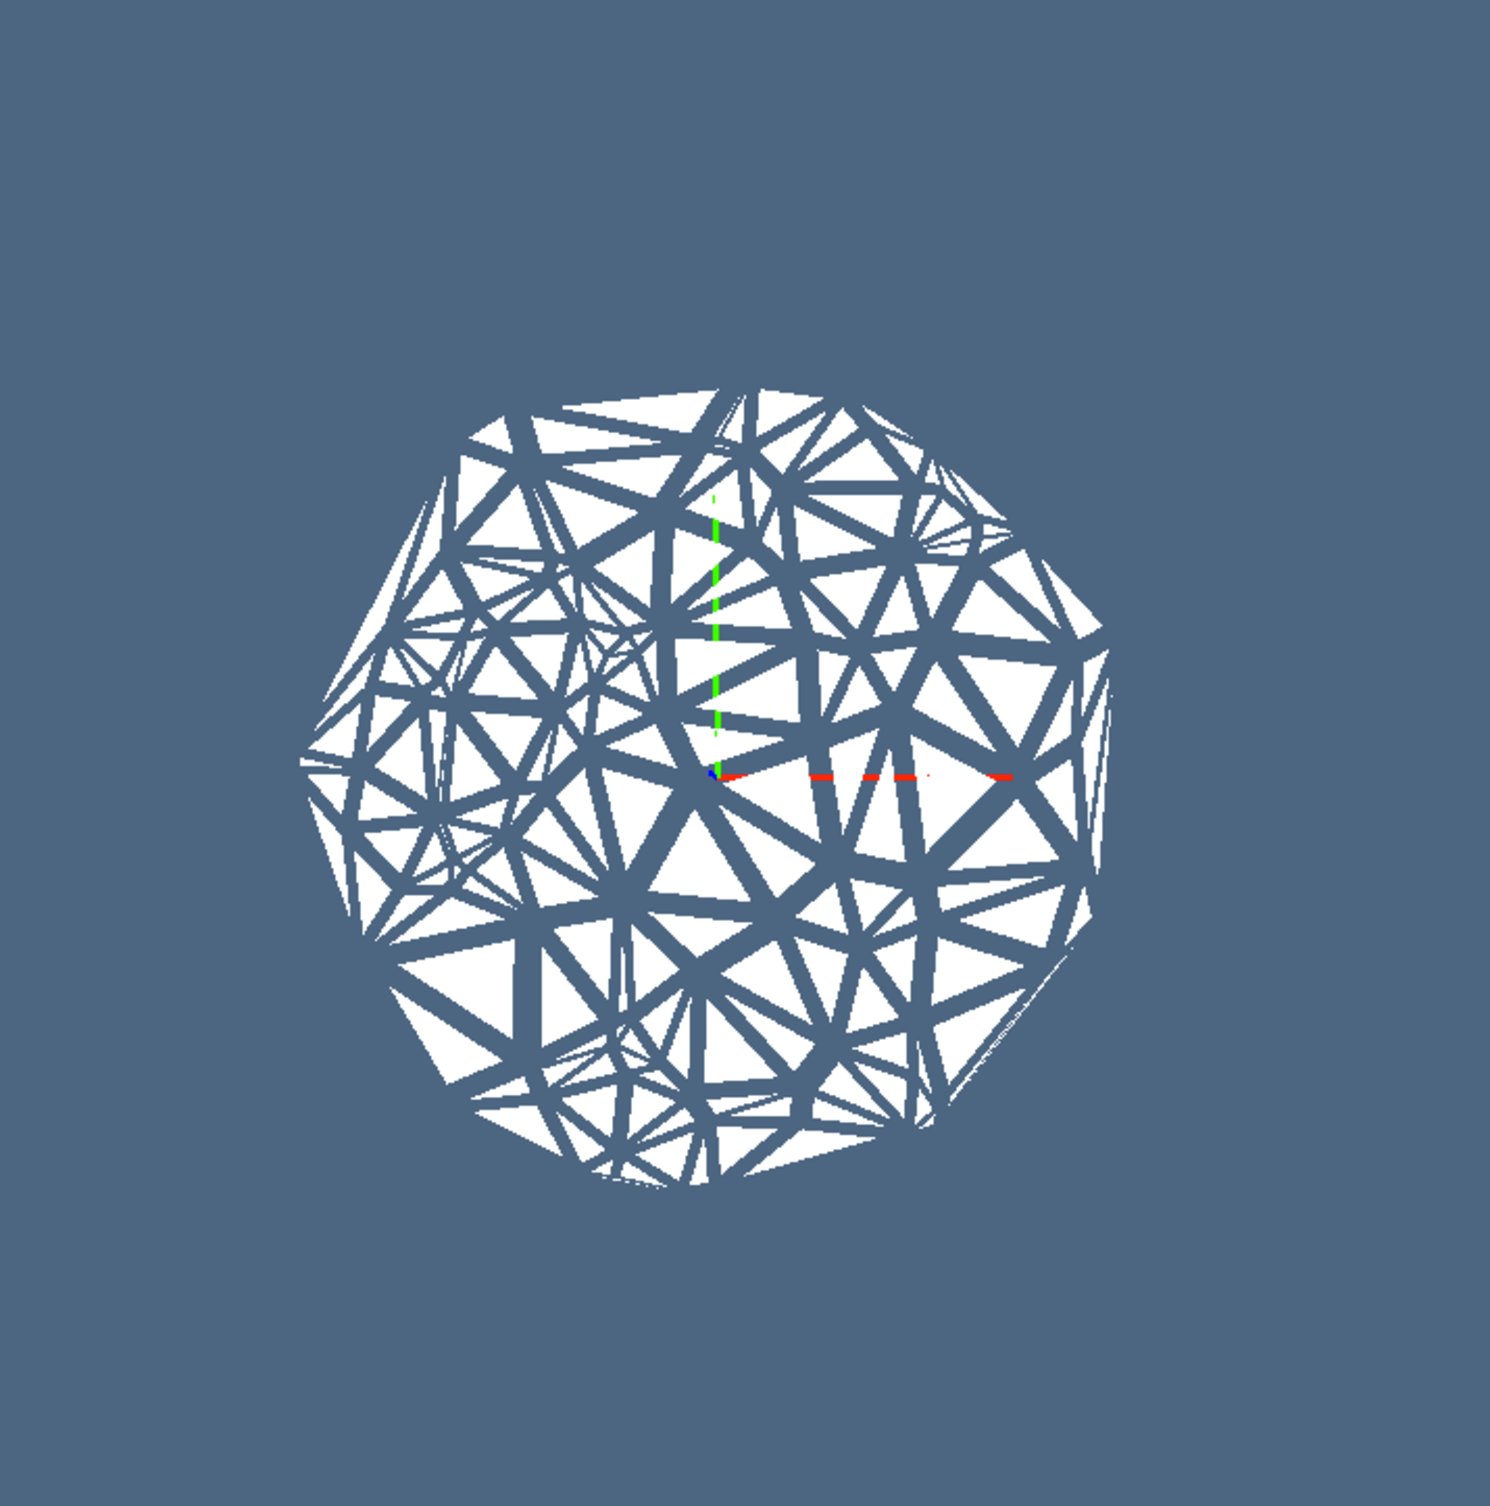
\includegraphics[height=0.245\linewidth,width=0.245\linewidth]{images/boolchain0a} 
   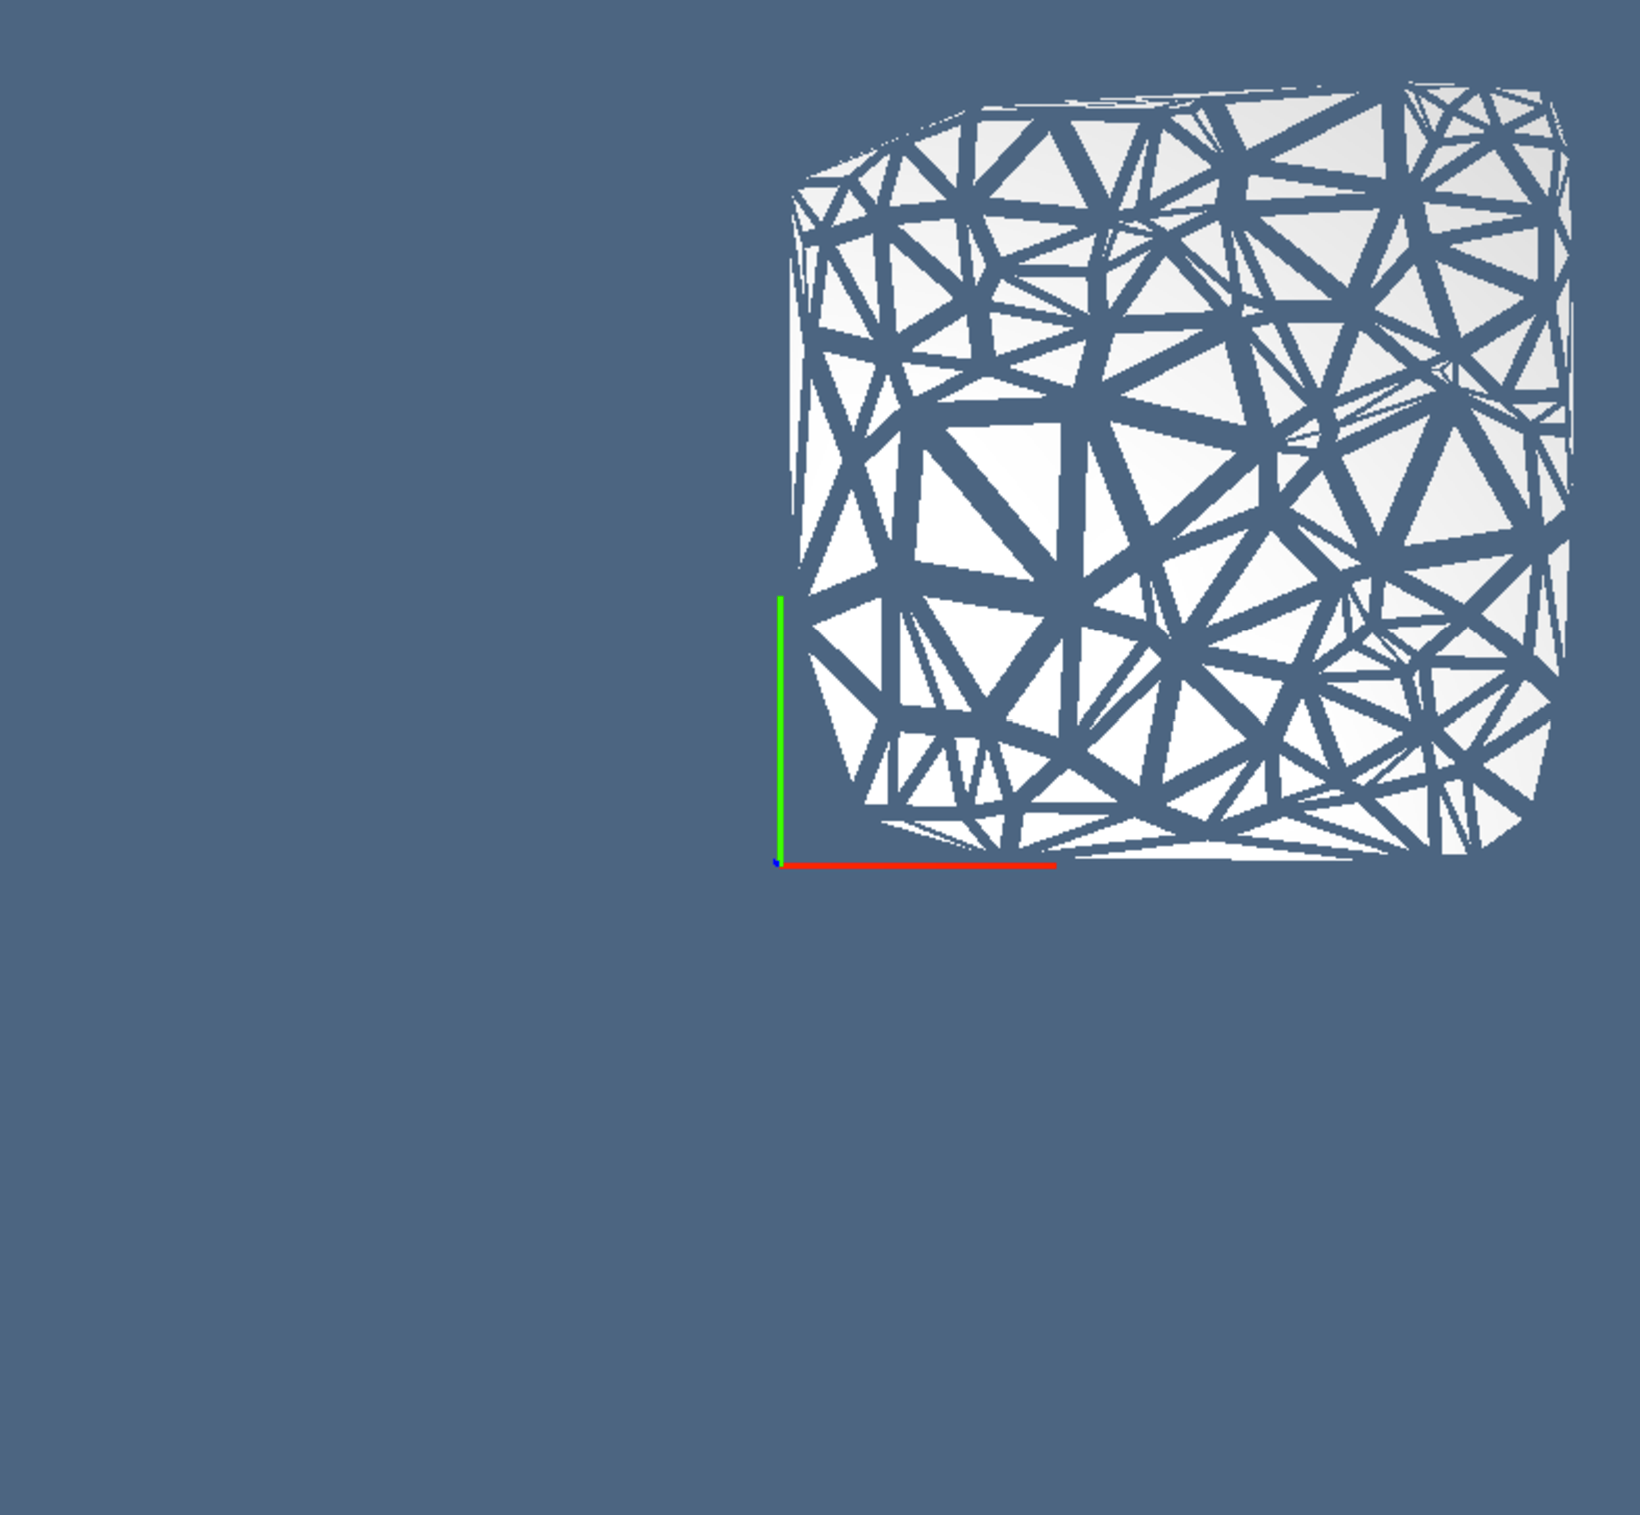
\includegraphics[height=0.245\linewidth,width=0.245\linewidth]{images/boolchain0b} 
   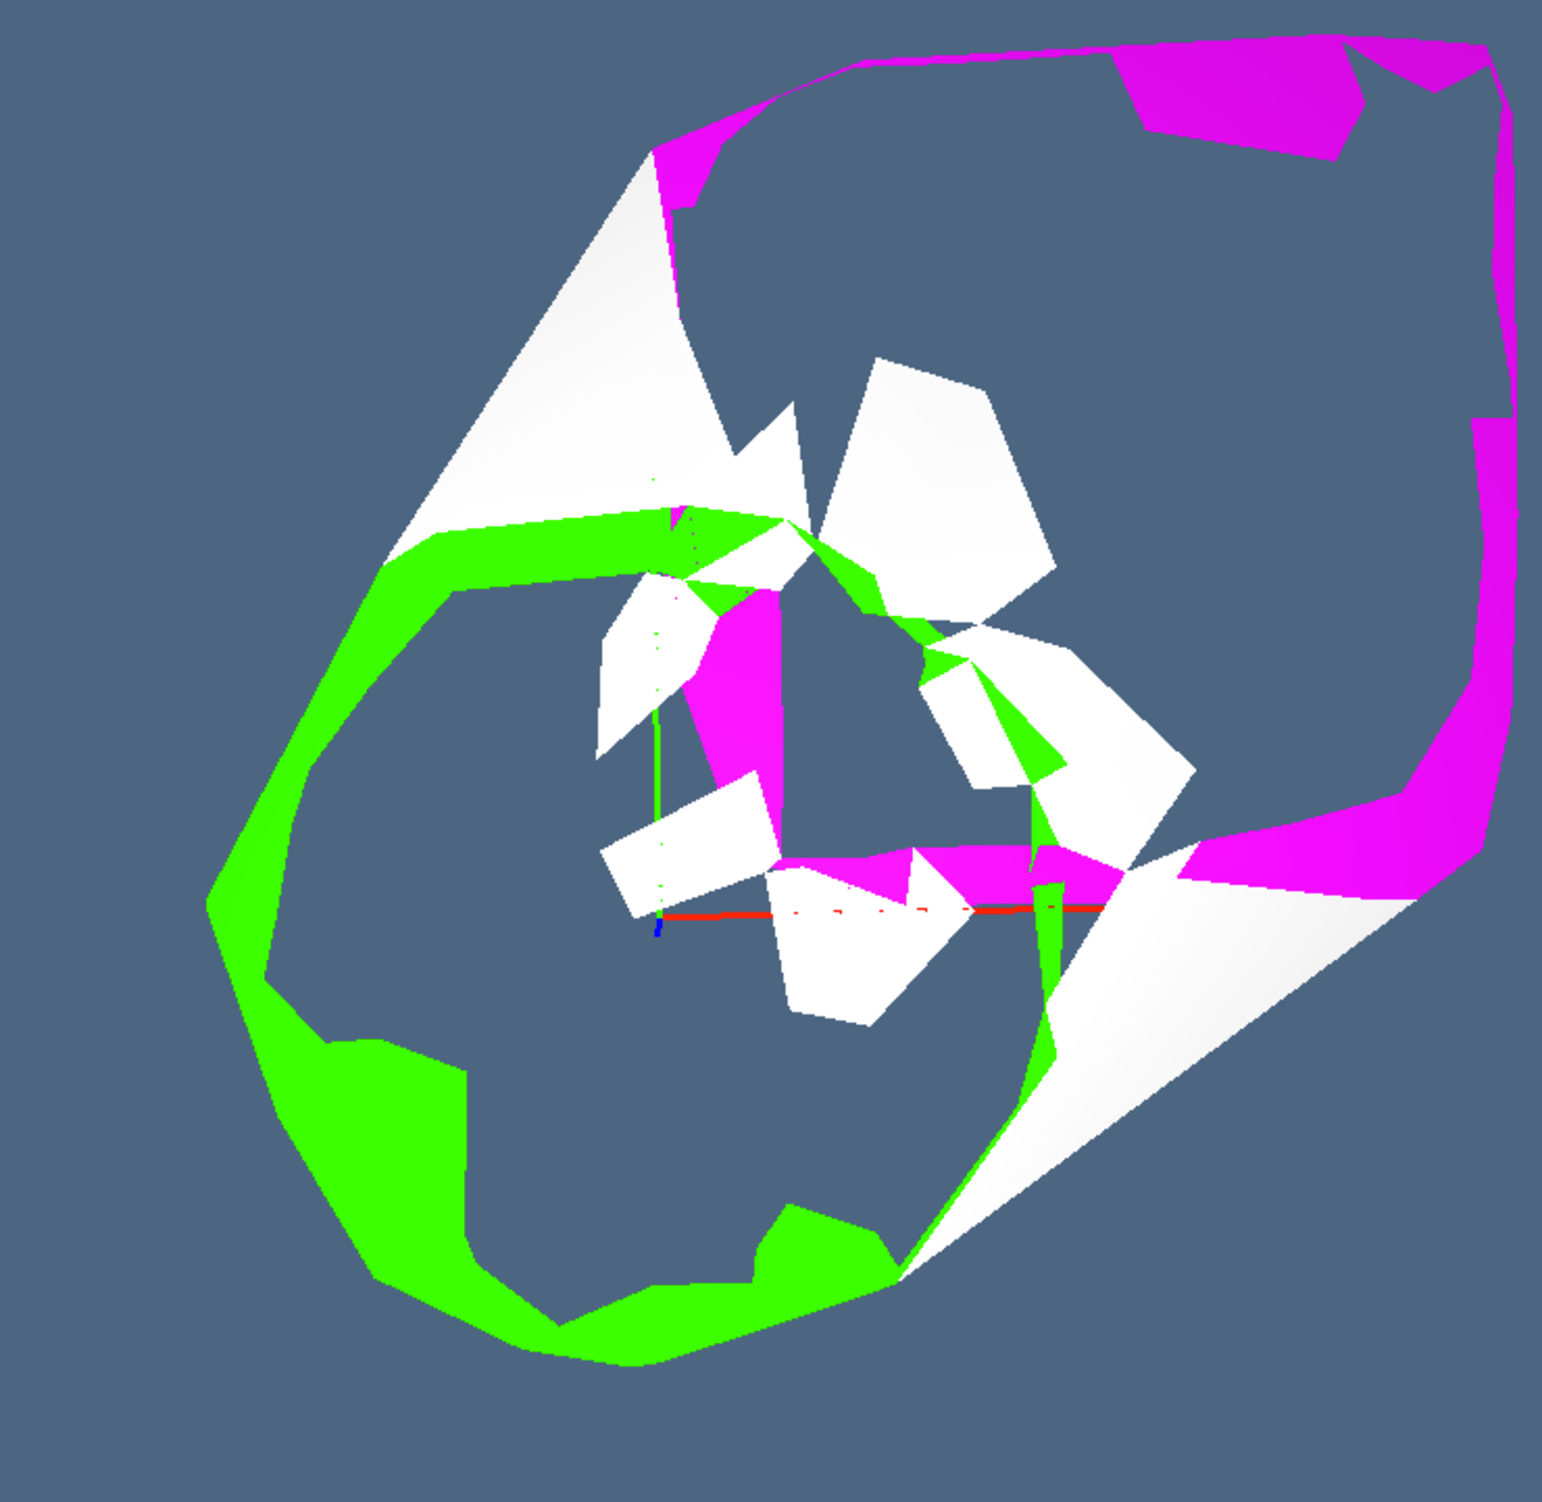
\includegraphics[height=0.245\linewidth,width=0.245\linewidth]{images/boolchain0c} 
   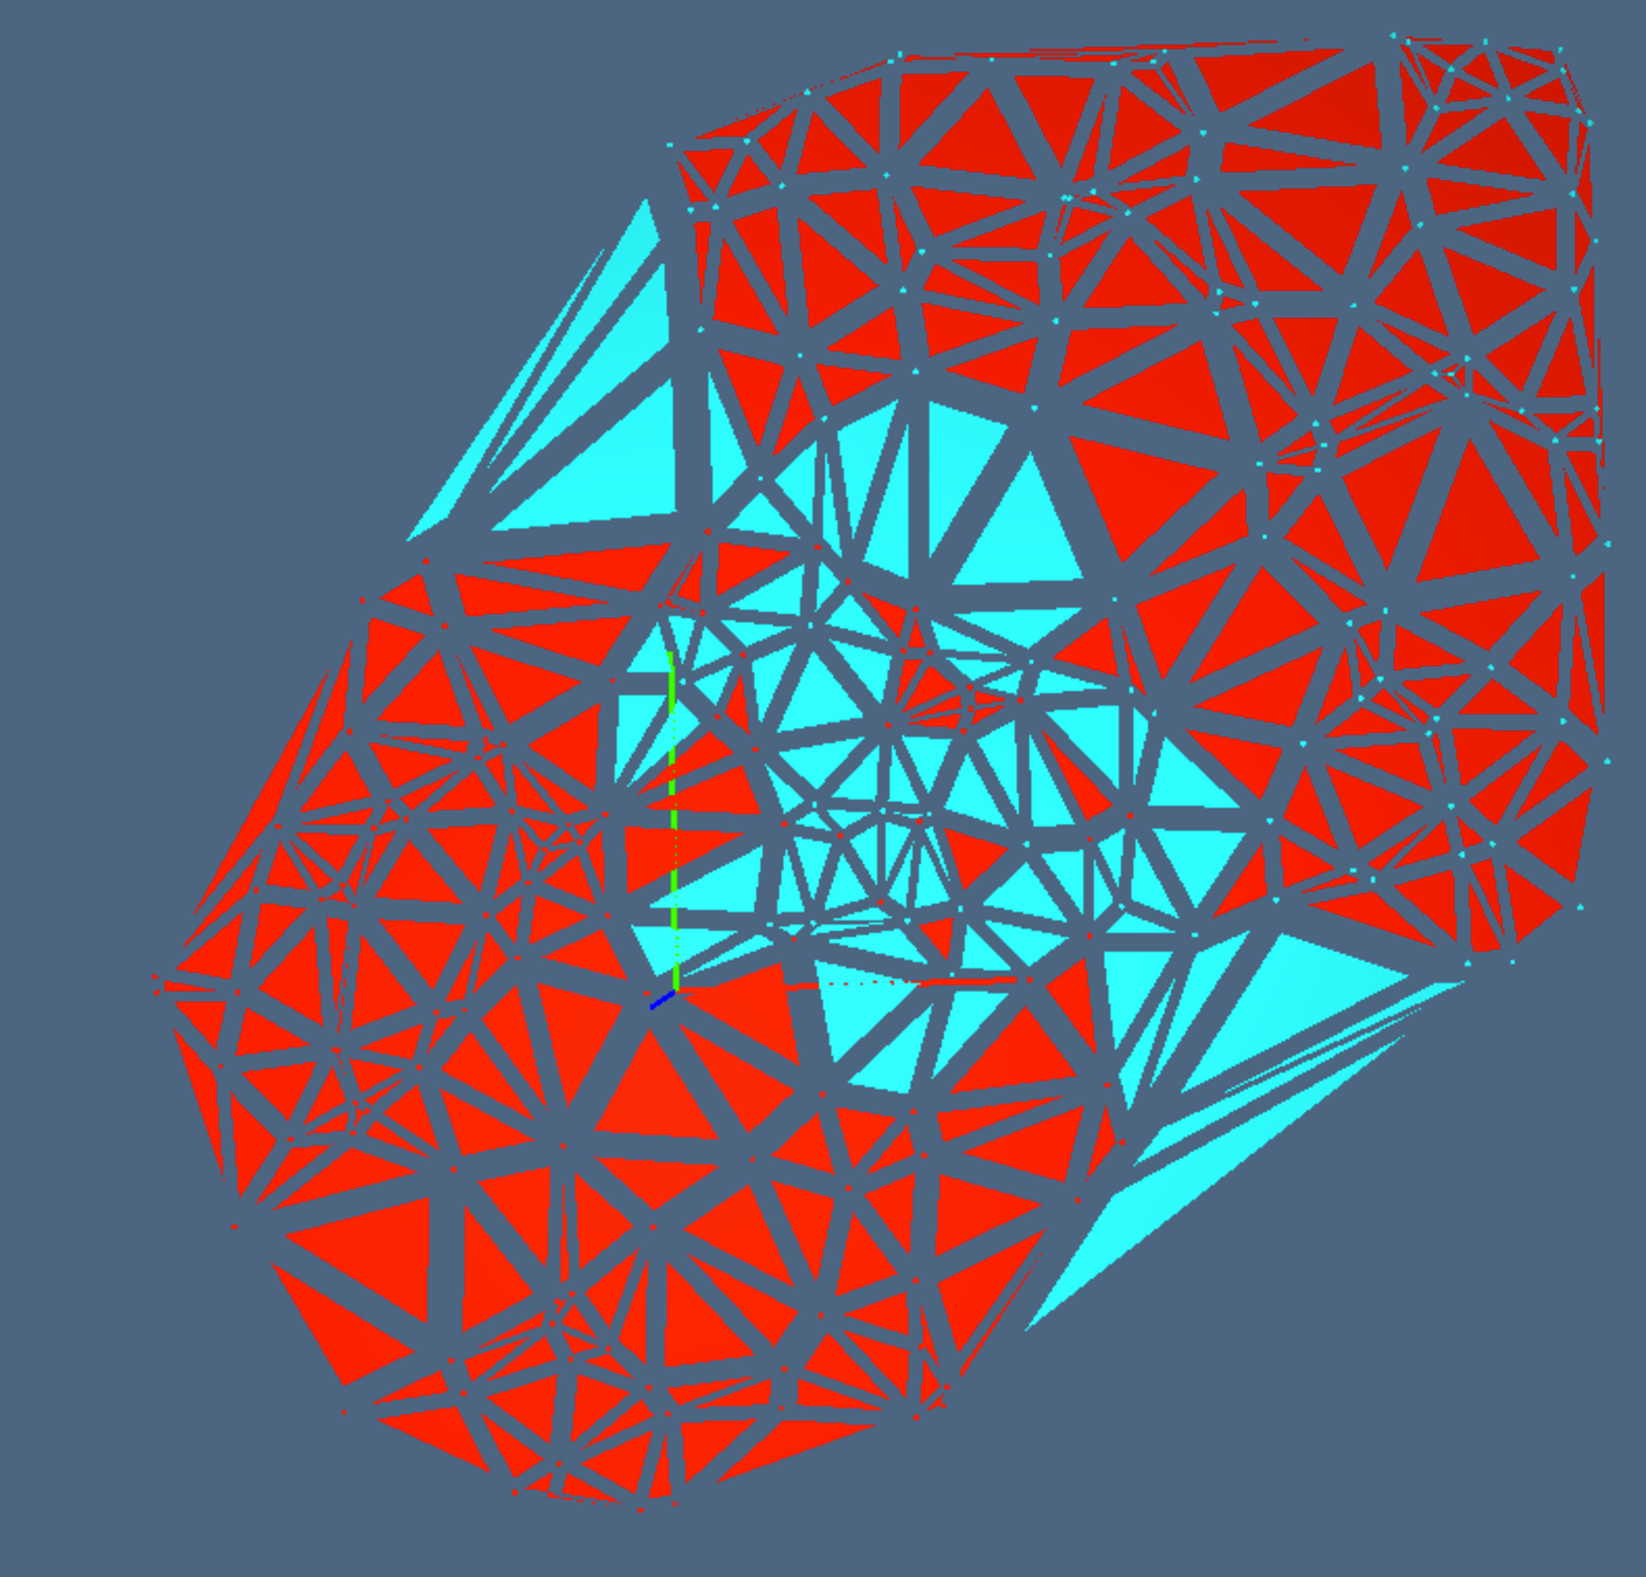
\includegraphics[height=0.245\linewidth,width=0.245\textwidth]{images/boolchain0d} 

   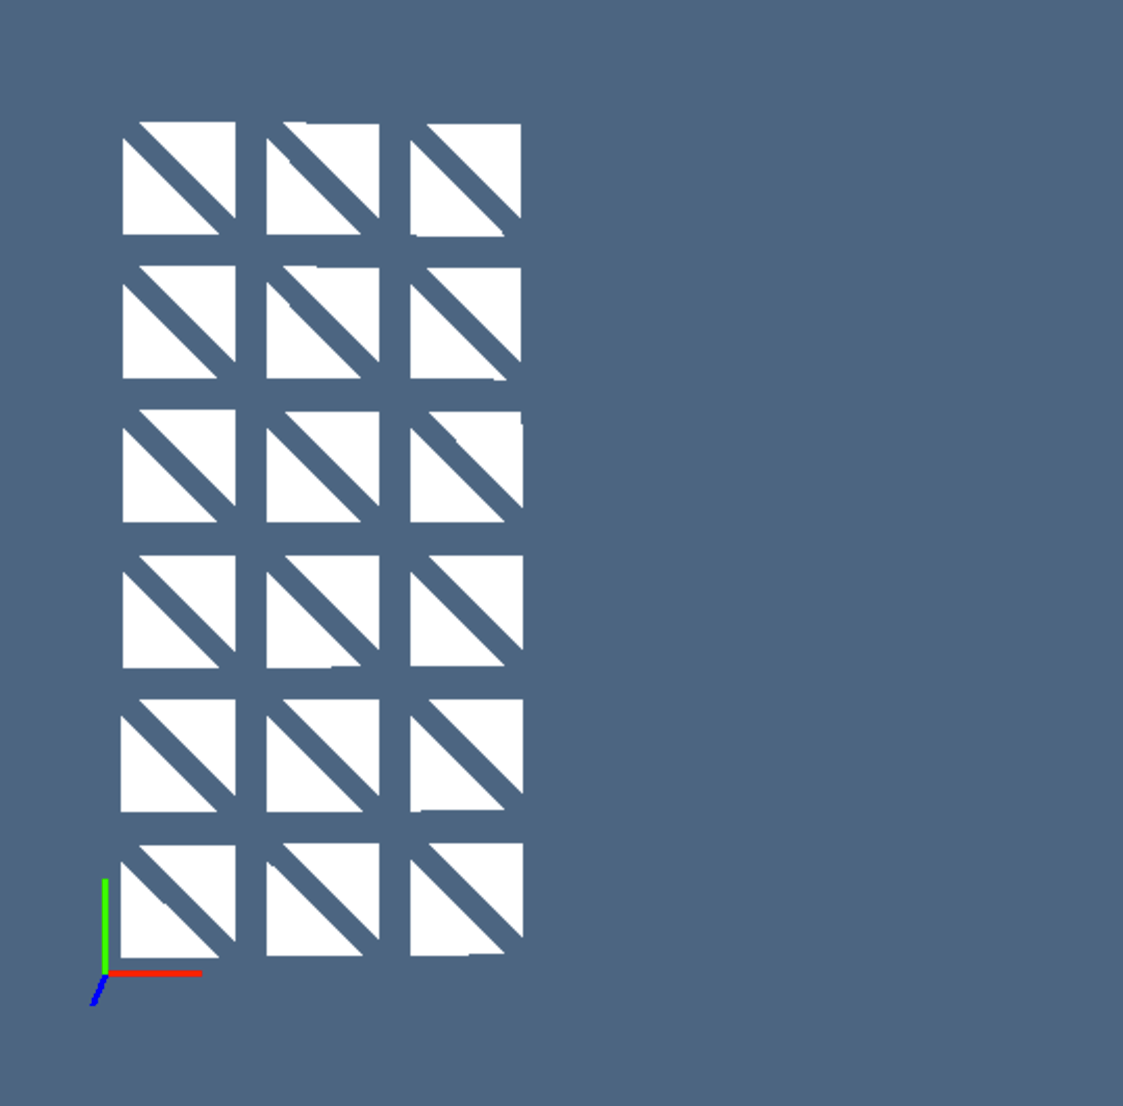
\includegraphics[height=0.245\linewidth,width=0.245\linewidth]{images/boolchain1a} 
   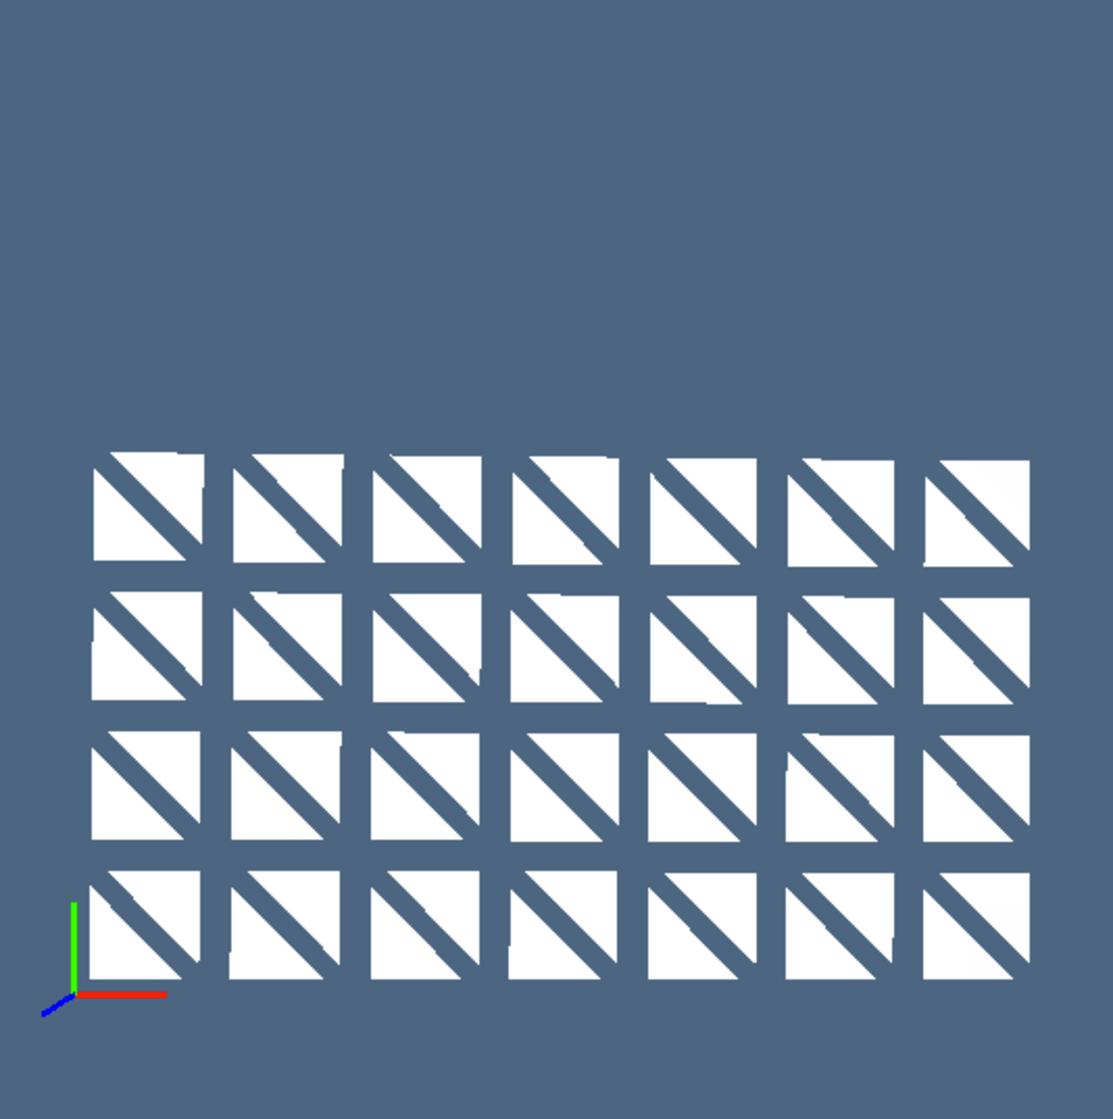
\includegraphics[height=0.245\linewidth,width=0.245\linewidth]{images/boolchain1b} 
   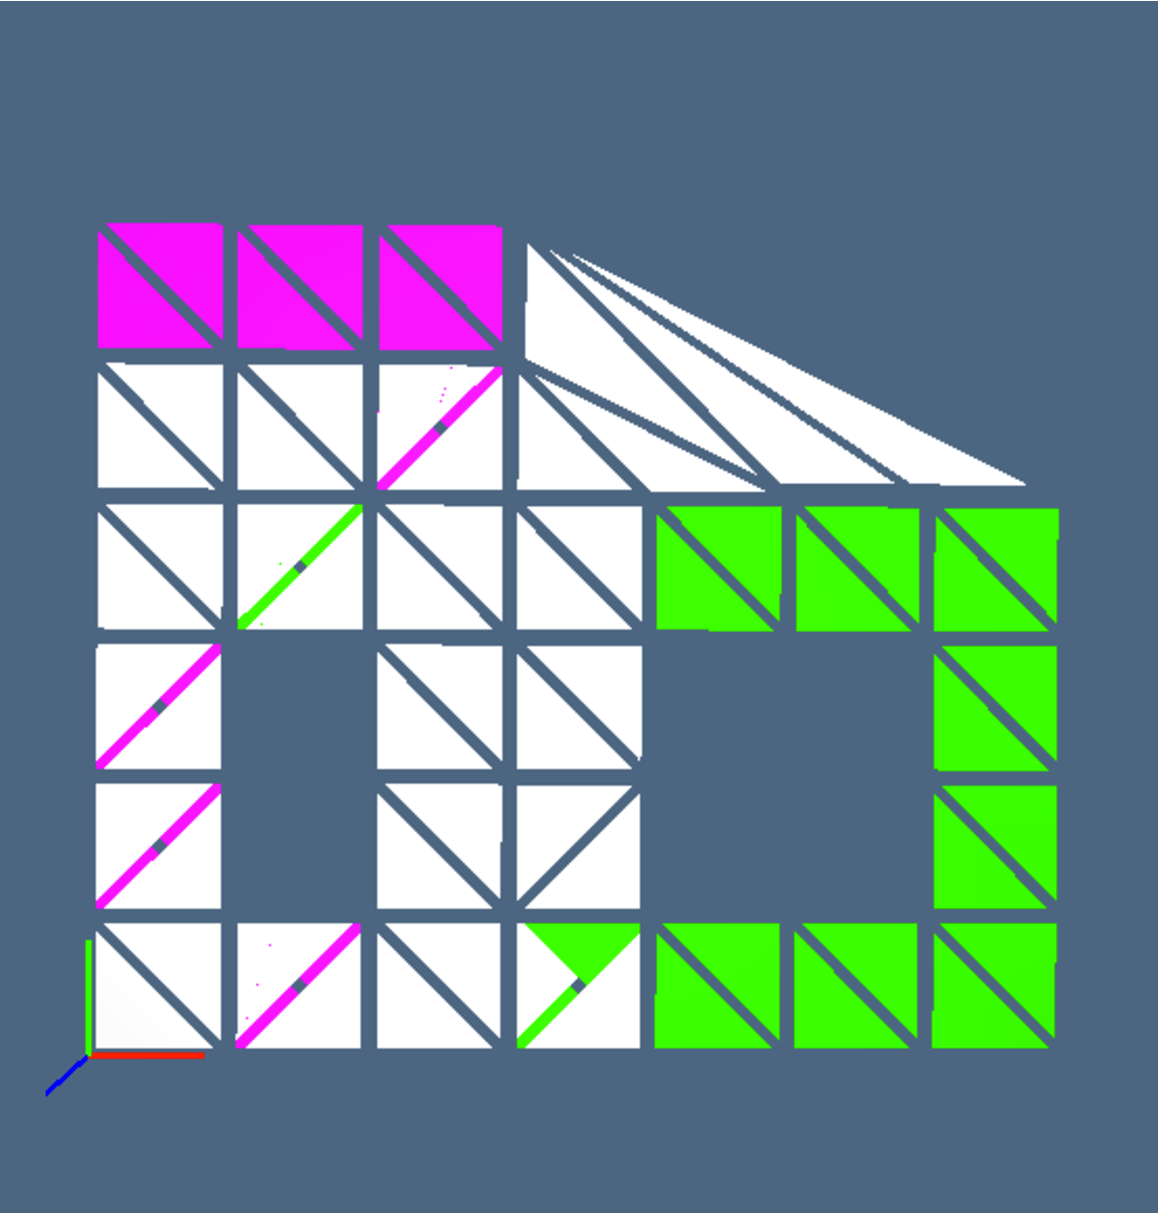
\includegraphics[height=0.245\linewidth,width=0.245\linewidth]{images/boolchain1c} 
   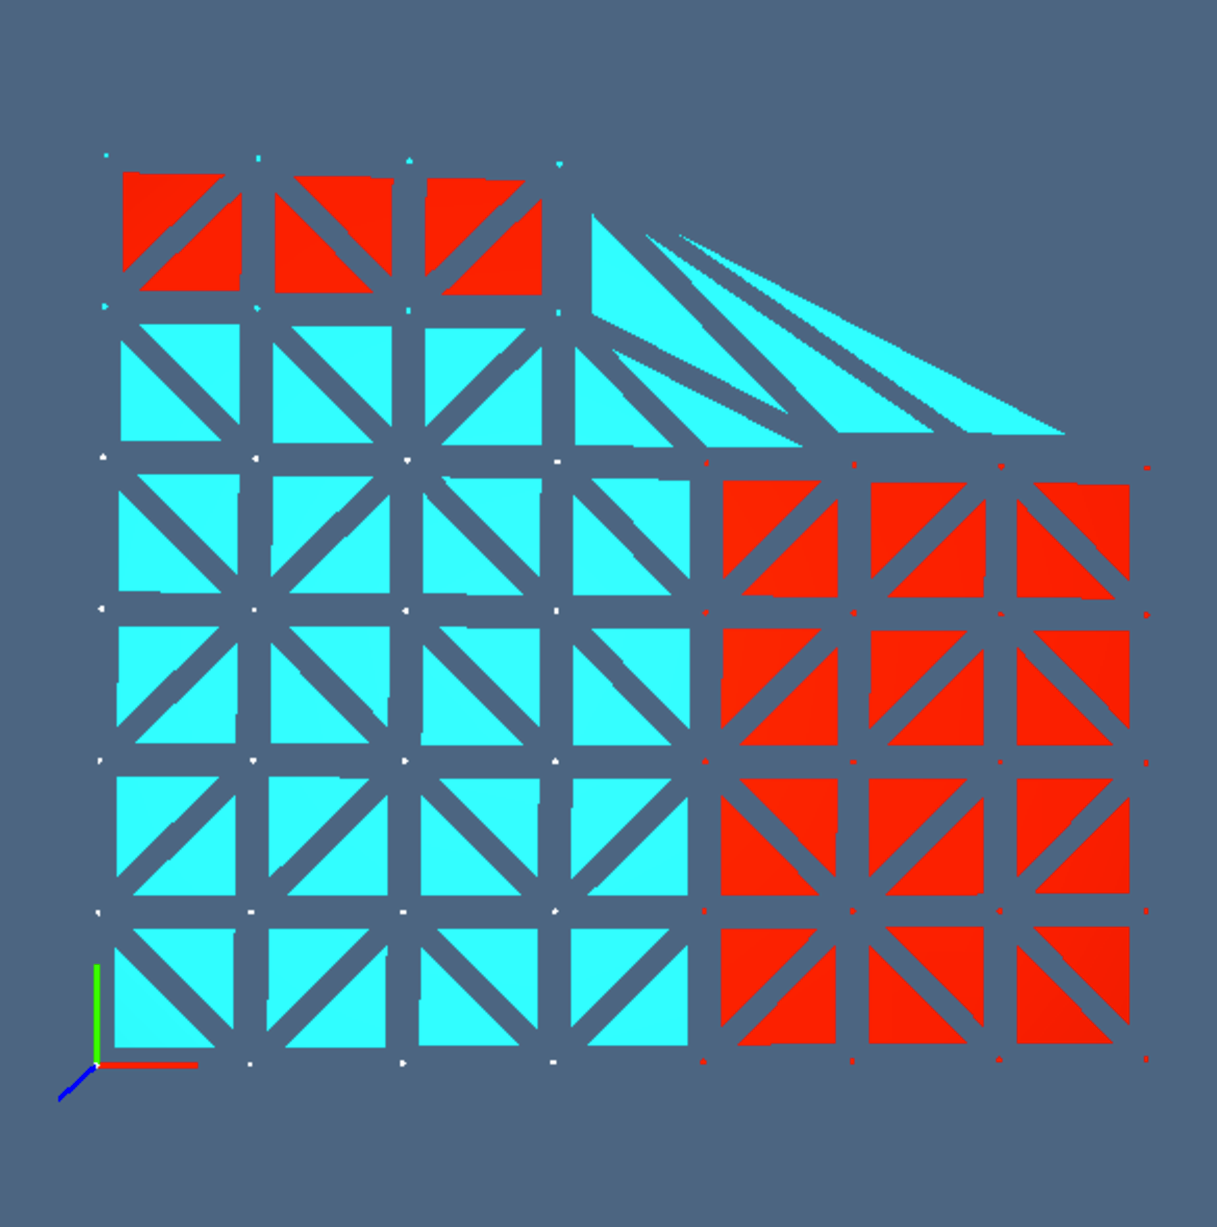
\includegraphics[height=0.245\linewidth,width=0.245\textwidth]{images/boolchain1d} 
   \caption{The selection of chains candidate to splitting, in both unstructured and structured meshes.}
   \label{fig:example}
\end{figure}


%>>>>>>>>>>>>>>>>>>>>>>>>>>>>>>>>>>>>>>>>>>>>>>>>>>>>>>>>>>>>>>>>>>>>>>>>>>>>>>>
\section{Splitting argument chains}
\label{sec:splitting}
%<<<<<<<<<<<<<<<<<<<<<<<<<<<<<<<<<<<<<<<<<<<<<<<<<<<<<<<<<<<<<<<<<<<<<<<<<<<<<<<

The \texttt{boolOps} function is the main procedure of the Boolean algorithm.
Its steps give an outline of the computations to be performed in sequence. The input LAR representations are first decomposed in their geometric and topological components, and embedded in the same space, so obtaining a global renumbering as \texttt{V}, \texttt{CV1}, \texttt{CV2}. Then the global Delaunay's triangulation \texttt{CV} and its set representation \texttt{setCV} are computed. In due order, the following steps are:  
\begin{enumerate}
\item 
the extraction of $\gamma^1,\gamma^2\subseteq\Lambda_d$, the coboundary of the boundaries of the Boolean arguments:
\[
\gamma^1 = (\delta_{d-1}\circ\partial_d) (\Lambda_d^1), \qquad
\gamma^2 = (\delta_{d-1}\circ\partial_d) (\Lambda_d^2);
\]  
\item 
the selection of the two invariant sub-chains, i.e.~of the subsets of $\Lambda_d^1, \Lambda_d^2$ that were not changed by the re-triangulation, and hence continue to contain some facets of the original boundaries:
\[
\gamma^{1'} \subseteq \gamma^1, \qquad
\gamma^{2'} \subseteq \gamma^2
\]
\end{enumerate}

\paragraph{The top-level algorithm}

%-------------------------------------------------------------------------------
\begin{flushleft} \small \label{scrap16}
\protect\makebox[0ex][r]{\NWtarget{nuweb10a}{\rule{0ex}{0ex}}\hspace{1em}}$\langle\,$Boolean subdivided complex\nobreak\ {\footnotesize 10a}$\,\rangle\equiv$
\vspace{-1ex}
\begin{list}{}{} \item
\mbox{}\verb@""" High level Boolean Application Programming Interface """@\\
\mbox{}\verb@@\hbox{$\langle\,$Minimal covering chains of divisors\nobreak\ {\footnotesize ?}$\,\rangle$}\verb@@\\
\mbox{}\verb@def boolOps(lar1,lar2):@\\
\mbox{}\verb@   (V1,CV1),(V2,CV2) = lar1,lar2@\\
\mbox{}\verb@   n1,n2 = len(V1),len(V2)@\\
\mbox{}\verb@   V, CV1, CV2, n12 = vertexSieve(lar1, lar2)@\\
\mbox{}\verb@   CV = Delaunay(array(V)).vertices@\\
\mbox{}\verb@   setCV = set([tuple(sorted(cell)) for cell in CV])@\\
\mbox{}\verb@   @\hbox{$\langle\,$Extraction of coboundary of boundary chains\nobreak\ {\footnotesize \NWlink{nuweb10b}{10b}}$\,\rangle$}\verb@@\\
\mbox{}\verb@   @\hbox{$\langle\,$Computation of invariant supercells\nobreak\ {\footnotesize \NWlink{nuweb11a}{11a}}$\,\rangle$}\verb@@\\
\mbox{}\verb@   @\hbox{$\langle\,$Invariant subsets of supercells\nobreak\ {\footnotesize \NWlink{nuweb11b}{11b}}$\,\rangle$}\verb@@\\
\mbox{}\verb@   @\hbox{$\langle\,$Minimal covering of divisors\nobreak\ {\footnotesize \NWlink{nuweb8a}{8a}}$\,\rangle$}\verb@@\\
\mbox{}\verb@   @\hbox{$\langle\,$Covers of divisors computation\nobreak\ {\footnotesize \NWlink{nuweb11c}{11c}}$\,\rangle$}\verb@@\\
\mbox{}\verb@   return V,n1,n2,n12, B1,B2@\\
\mbox{}\verb@@{\NWsep}
\end{list}
\vspace{-1ex}
\footnotesize\addtolength{\baselineskip}{-1ex}
\begin{list}{}{\setlength{\itemsep}{-\parsep}\setlength{\itemindent}{-\leftmargin}}
\item \NWtxtMacroRefIn\ \NWlink{nuweb13a}{13a}.
\end{list}
\end{flushleft}
%-------------------------------------------------------------------------------

\paragraph{Extraction of coboundary of boundary chains}

After the embedding of the two topologies in the same coordinate space and the Delaunay's re-triangulation, the two $\gamma^1,\gamma^2$ $d$-chains are computed by the following macro, and stored in the \texttt{BSupCells1} and \texttt{BSupCells2} variables.

%-------------------------------------------------------------------------------
\begin{flushleft} \small \label{scrap17}
\protect\makebox[0ex][r]{\NWtarget{nuweb10b}{\rule{0ex}{0ex}}\hspace{1em}}$\langle\,$Extraction of coboundary of boundary chains\nobreak\ {\footnotesize 10b}$\,\rangle\equiv$
\vspace{-1ex}
\begin{list}{}{} \item
\mbox{}\verb@# Second stage of Boolean algorithm@\\
\mbox{}\verb@B1,B2 = boundaryVertices( V, CV1, CV2 )@\\
\mbox{}\verb@# Extraction of coboundary of boundary chains@\\
\mbox{}\verb@BSupCells1 = boundarySuperCells( V, CV1 )@\\
\mbox{}\verb@BSupCells2 = boundarySuperCells( V, CV2 )@\\
\mbox{}\verb@@\\
\mbox{}\verb@VIEW(STRUCT([ @\\
\mbox{}\verb@   COLOR(GREEN)(STRUCT(MKPOLS(((V,[CV1[c] for c in BSupCells1]))))), @\\
\mbox{}\verb@   COLOR(MAGENTA)(STRUCT(MKPOLS(((V,[CV2[c] for c in BSupCells2]))))) @\\
\mbox{}\verb@])) @\\
\mbox{}\verb@@{\NWsep}
\end{list}
\vspace{-1ex}
\footnotesize\addtolength{\baselineskip}{-1ex}
\begin{list}{}{\setlength{\itemsep}{-\parsep}\setlength{\itemindent}{-\leftmargin}}
\item \NWtxtMacroRefIn\ \NWlink{nuweb10a}{10a}.
\end{list}
\end{flushleft}
%-------------------------------------------------------------------------------

\paragraph{Invariant subsets of supercells}

Then the sub-chains $\gamma^{1'},\gamma^{2'}$ (those not changed by the Boolean merging) are computed by the \texttt{invariantSuperCells} function, and stored in \texttt{invSupCells1} and \texttt{invSupCells2} variables, in order to compute, by chain difference, the \texttt{divisor1} and \texttt{divisor2} $d$-chains.

%-------------------------------------------------------------------------------
\begin{flushleft} \small \label{scrap18}
\protect\makebox[0ex][r]{\NWtarget{nuweb11a}{\rule{0ex}{0ex}}\hspace{1em}}$\langle\,$Computation of invariant supercells\nobreak\ {\footnotesize 11a}$\,\rangle\equiv$
\vspace{-1ex}
\begin{list}{}{} \item
\mbox{}\verb@def invariantSuperCells(V,BSupCells1,CV1,setCV):@\\
\mbox{}\verb@   out = []@\\
\mbox{}\verb@   for cell in BSupCells1:@\\
\mbox{}\verb@      if tuple(CV1[cell]) in setCV: out += [cell]@\\
\mbox{}\verb@   return out@\\
\mbox{}\verb@@{\NWsep}
\end{list}
\vspace{-1ex}
\footnotesize\addtolength{\baselineskip}{-1ex}
\begin{list}{}{\setlength{\itemsep}{-\parsep}\setlength{\itemindent}{-\leftmargin}}
\item \NWtxtMacroRefIn\ \NWlink{nuweb10a}{10a}.
\end{list}
\end{flushleft}
%-------------------------------------------------------------------------------

%-------------------------------------------------------------------------------
\begin{flushleft} \small \label{scrap19}
\protect\makebox[0ex][r]{\NWtarget{nuweb11b}{\rule{0ex}{0ex}}\hspace{1em}}$\langle\,$Invariant subsets of supercells\nobreak\ {\footnotesize 11b}$\,\rangle\equiv$
\vspace{-1ex}
\begin{list}{}{} \item
\mbox{}\verb@# Invariant subsets of supercells@\\
\mbox{}\verb@invSupCells1 = invariantSuperCells(V,BSupCells1,CV1,setCV)@\\
\mbox{}\verb@invSupCells2 = invariantSuperCells(V,BSupCells2,CV2,setCV)@\\
\mbox{}\verb@@\\
\mbox{}\verb@divisor1 = set(BSupCells1).difference(invSupCells1)@\\
\mbox{}\verb@divisor2 = set(BSupCells2).difference(invSupCells2)@\\
\mbox{}\verb@VIEW(STRUCT([ @\\
\mbox{}\verb@   COLOR(GREEN)(STRUCT(MKPOLS(((V,[CV1[c] for c in divisor1]))))), @\\
\mbox{}\verb@   COLOR(MAGENTA)(STRUCT(MKPOLS(((V,[CV2[c] for c in divisor2]))))) @\\
\mbox{}\verb@]))@\\
\mbox{}\verb@@{\NWsep}
\end{list}
\vspace{-1ex}
\footnotesize\addtolength{\baselineskip}{-1ex}
\begin{list}{}{\setlength{\itemsep}{-\parsep}\setlength{\itemindent}{-\leftmargin}}
\item \NWtxtMacroRefIn\ \NWlink{nuweb10a}{10a}.
\end{list}
\end{flushleft}
%-------------------------------------------------------------------------------
\paragraph{Covers of divisors computation}
%-------------------------------------------------------------------------------
\begin{flushleft} \small \label{scrap20}
\protect\makebox[0ex][r]{\NWtarget{nuweb11c}{\rule{0ex}{0ex}}\hspace{1em}}$\langle\,$Covers of divisors computation\nobreak\ {\footnotesize 11c}$\,\rangle\equiv$
\vspace{-1ex}
\begin{list}{}{} \item
\mbox{}\verb@@\\
\mbox{}\verb@# Covers of divisors computation@\\
\mbox{}\verb@covers1 = minimalCovers(V,divisor1,CV1,CV,setCV)@\\
\mbox{}\verb@covers2 = minimalCovers(V,divisor2,CV2,CV,setCV)   @\\
\mbox{}\verb@VIEW(STRUCT([ @\\
\mbox{}\verb@   EXPLODE(1.2,1.2,1)(MKPOLS(((V,CV)))), @\\
\mbox{}\verb@   COLOR(GREEN)(EXPLODE(1.2,1.2,1)(MKPOLS(((V,[CV[c] for c in CAT(covers1)]))))), @\\
\mbox{}\verb@   COLOR(MAGENTA)(EXPLODE(1.2,1.2,1)(MKPOLS(((V,[CV[c] for c in CAT(covers2)])))))@\\
\mbox{}\verb@    ]))@\\
\mbox{}\verb@@{\NWsep}
\end{list}
\vspace{-1ex}
\footnotesize\addtolength{\baselineskip}{-1ex}
\begin{list}{}{\setlength{\itemsep}{-\parsep}\setlength{\itemindent}{-\leftmargin}}
\item \NWtxtMacroRefIn\ \NWlink{nuweb10a}{10a}.
\end{list}
\end{flushleft}
%-------------------------------------------------------------------------------


%-------------------------------------------------------------------------------
\subsection{Matching cells in $\Sigma_\cap$ with spanning chains in $\Lambda^1$, $\Lambda^2$}
%-------------------------------------------------------------------------------

The next step of the \emph{Boolean Chains} algorithm retrieves and compare the chains of $d$-cells incident on $\texttt{V}(\partial_d(\Lambda^1)), \texttt{V}(\partial_d(\Lambda^2))$ and on $\texttt{V}(\partial_d(\Sigma^\cap))$. A filtering step working in $O(n)$ is performed in regard to this.

\paragraph{Filtering cells incident on a subset of vertices}

The selection of the $d$-chain incident on a $0$-chain (subset of vertices) can be executed either in time roughly proportional to the output, via a SpMV multiplication of the $\texttt{CV} := \texttt{CSR}(M_d)$ matrix times the (binary) coordinate representation of the $0$-chain, or in time proportional to the input, via a more traditional select filtering of cells in a \texttt{CV} table, with respect to the subset of vertices.


%-------------------------------------------------------------------------------
\begin{flushleft} \small \label{scrap21}
\protect\makebox[0ex][r]{\NWtarget{nuweb12}{\rule{0ex}{0ex}}\hspace{1em}}$\langle\,$Select cells incident on vertices\nobreak\ {\footnotesize 12}$\,\rangle\equiv$
\vspace{-1ex}
\begin{list}{}{} \item
\mbox{}\verb@""" Select the $d$-chain incident on a $0$-chain """@\\
\mbox{}\verb@def selectIncidentChain( V, CV ):@\\
\mbox{}\verb@   def selectIncidentChain0( v ):@\\
\mbox{}\verb@      return [k for k in range(len(CV)) if v in CV[k] ]@\\
\mbox{}\verb@   return selectIncidentChain0@\\
\mbox{}\verb@@{\NWsep}
\end{list}
\vspace{-1ex}
\footnotesize\addtolength{\baselineskip}{-1ex}
\begin{list}{}{\setlength{\itemsep}{-\parsep}\setlength{\itemindent}{-\leftmargin}}
\item \NWtxtMacroRefIn\ \NWlink{nuweb13a}{13a}.
\end{list}
\end{flushleft}
%-------------------------------------------------------------------------------


%-------------------------------------------------------------------------------
\subsection{Splitting cells}
%-------------------------------------------------------------------------------
%-------------------------------------------------------------------------------
\subsection{Keeping cell dictionaries updated}
%-------------------------------------------------------------------------------
%>>>>>>>>>>>>>>>>>>>>>>>>>>>>>>>>>>>>>>>>>>>>>>>>>>>>>>>>>>>>>>>>>>>>>>>>>>>>>>>
\section{Boolean outputs computations}
%<<<<<<<<<<<<<<<<<<<<<<<<<<<<<<<<<<<<<<<<<<<<<<<<<<<<<<<<<<<<<<<<<<<<<<<<<<<<<<<
%>>>>>>>>>>>>>>>>>>>>>>>>>>>>>>>>>>>>>>>>>>>>>>>>>>>>>>>>>>>>>>>>>>>>>>>>>>>>>>>
\section{Export the boolean module}
%<<<<<<<<<<<<<<<<<<<<<<<<<<<<<<<<<<<<<<<<<<<<<<<<<<<<<<<<<<<<<<<<<<<<<<<<<<<<<<<

The \texttt{boolean.py} module is exported to the library \texttt{lar-cc/lib}. Therefore many of the macros developed in this module are expanded and written to an external file.

%------------------------------------------------------------------
\begin{flushleft} \small
\begin{minipage}{\linewidth} \label{scrap22}
\protect\makebox[0ex][r]{\NWtarget{nuweb13a}{\rule{0ex}{0ex}}\hspace{1em}}\verb@"lib/py/boolean2.py"@\nobreak\ {\footnotesize 13a }$\equiv$
\vspace{-1ex}
\begin{list}{}{} \item
\mbox{}\verb@""" Module with Boolean operators using chains and CSR matrices """@\\
\mbox{}\verb@@\hbox{$\langle\,$Initial import of modules\nobreak\ {\footnotesize \NWlink{nuweb17b}{17b}}$\,\rangle$}\verb@@\\
\mbox{}\verb@@\hbox{$\langle\,$Symbolic utility to represent points as strings\nobreak\ {\footnotesize \NWlink{nuweb18b}{18b}}$\,\rangle$}\verb@@\\
\mbox{}\verb@@\hbox{$\langle\,$Affine transformations of $n$ points\nobreak\ {\footnotesize \NWlink{nuweb18a}{18a}}$\,\rangle$}\verb@@\\
\mbox{}\verb@@\hbox{$\langle\,$Generation of $n$ random points in the unit $d$-disk\nobreak\ {\footnotesize \NWlink{nuweb13b}{13b}}$\,\rangle$}\verb@@\\
\mbox{}\verb@@\hbox{$\langle\,$Generation of $n$ random points in the standard $d$-cuboid\nobreak\ {\footnotesize \NWlink{nuweb14a}{14a}}$\,\rangle$}\verb@@\\
\mbox{}\verb@@\hbox{$\langle\,$Triangulation of random points\nobreak\ {\footnotesize \NWlink{nuweb14b}{14b}}$\,\rangle$}\verb@@\\
\mbox{}\verb@@\hbox{$\langle\,$Boolean subdivided complex\nobreak\ {\footnotesize \NWlink{nuweb10a}{10a}}$\,\rangle$}\verb@@\\
\mbox{}\verb@@\hbox{$\langle\,$High-level boolean operations\nobreak\ {\footnotesize \NWlink{nuweb2}{2}}$\,\rangle$}\verb@@\\
\mbox{}\verb@@\hbox{$\langle\,$Place the vertices of Boolean arguments in a common space\nobreak\ {\footnotesize \NWlink{nuweb3a}{3a}}$\,\rangle$}\verb@@\\
\mbox{}\verb@@\hbox{$\langle\,$Show vertices of arguments\nobreak\ {\footnotesize ?}$\,\rangle$}\verb@@\\
\mbox{}\verb@@\hbox{$\langle\,$Compute boundary vertices of both arguments\nobreak\ {\footnotesize \NWlink{nuweb8b}{8b}}$\,\rangle$}\verb@@\\
\mbox{}\verb@@\hbox{$\langle\,$Select cells incident on vertices\nobreak\ {\footnotesize \NWlink{nuweb12}{12}}$\,\rangle$}\verb@@\\
\mbox{}\verb@@\hbox{$\langle\,$Compute the $d$-cells in the coboundary of boundary\nobreak\ {\footnotesize \NWlink{nuweb7a}{7a}}$\,\rangle$}\verb@@\\
\mbox{}\verb@@\hbox{$\langle\,$Compute the boundary divisors of both arguments\nobreak\ {\footnotesize \NWlink{nuweb7b}{7b}}$\,\rangle$}\verb@@\\
\mbox{}\verb@@\hbox{$\langle\,$Visualization of a subset of cells\nobreak\ {\footnotesize \NWlink{nuweb16e}{16e}}$\,\rangle$}\verb@@\\
\mbox{}\verb@@{\NWsep}
\end{list}
\vspace{-2ex}
\end{minipage}\\[4ex]
\end{flushleft}
%------------------------------------------------------------------

%>>>>>>>>>>>>>>>>>>>>>>>>>>>>>>>>>>>>>>>>>>>>>>>>>>>>>>>>>>>>>>>>>>>>>>>>>>>>>>>
\section{Tests}
%<<<<<<<<<<<<<<<<<<<<<<<<<<<<<<<<<<<<<<<<<<<<<<<<<<<<<<<<<<<<<<<<<<<<<<<<<<<<<<<
%-------------------------------------------------------------------------------
\subsection{Generation of random data}

We found useful to drive the development of new modules using randomly generated data, so that every upcoming execution of the developed algorithms is naturally driven to be challenged by different data.

\subsubsection{Testing the main algorithm}

\paragraph{Write the test executable file}




\subsubsection{Lowest-level space generation procedures}

\paragraph{Random points in unit disk} 
First we generate a  set of $n$ random points in the unit $D^d$ disk centred on the origin, to be subsequently used to generate a random Delaunay complex of variable granularity.

%------------------------------------------------------------------
\begin{flushleft} \small \label{scrap23}
\protect\makebox[0ex][r]{\NWtarget{nuweb13b}{\rule{0ex}{0ex}}\hspace{1em}}$\langle\,$Generation of $n$ random points in the unit $d$-disk\nobreak\ {\footnotesize 13b}$\,\rangle\equiv$
\vspace{-1ex}
\begin{list}{}{} \item
\mbox{}\verb@def randomPointsInUnitCircle(n=200,d=2, r=1):@\\
\mbox{}\verb@   points = random.random((n,d)) * ([2*math.pi]+[1]*(d-1))@\\
\mbox{}\verb@   return [[SQRT(p[1])*COS(p[0]),SQRT(p[1])*SIN(p[0])] for p in points]@\\
\mbox{}\verb@   ## TODO: correct for $d$-sphere@\\
\mbox{}\verb@@\\
\mbox{}\verb@if __name__=="__main__":@\\
\mbox{}\verb@   VIEW(STRUCT(AA(MK)(randomPointsInUnitCircle()))) @\\
\mbox{}\verb@@{\NWsep}
\end{list}
\vspace{-1ex}
\footnotesize\addtolength{\baselineskip}{-1ex}
\begin{list}{}{\setlength{\itemsep}{-\parsep}\setlength{\itemindent}{-\leftmargin}}
\item \NWtxtMacroRefIn\ \NWlink{nuweb13a}{13a}.
\end{list}
\end{flushleft}
%------------------------------------------------------------------

\paragraph{Random points in the standard $d$-cuboid} 
A set of $n$ random $d$-points is then generated within the standard $d$-cuboid, i.e.~withing the $d$-dimensional interval with a vertex on the origin.

%------------------------------------------------------------------
\begin{flushleft} \small \label{scrap24}
\protect\makebox[0ex][r]{\NWtarget{nuweb14a}{\rule{0ex}{0ex}}\hspace{1em}}$\langle\,$Generation of $n$ random points in the standard $d$-cuboid\nobreak\ {\footnotesize 14a}$\,\rangle\equiv$
\vspace{-1ex}
\begin{list}{}{} \item
\mbox{}\verb@def randomPointsInUnitCuboid(n=200,d=2):@\\
\mbox{}\verb@   return random.random((n,d)).tolist()@\\
\mbox{}\verb@@\\
\mbox{}\verb@if __name__=="__main__":@\\
\mbox{}\verb@   VIEW(STRUCT(AA(MK)(randomPointsInUnitCuboid()))) @\\
\mbox{}\verb@@{\NWsep}
\end{list}
\vspace{-1ex}
\footnotesize\addtolength{\baselineskip}{-1ex}
\begin{list}{}{\setlength{\itemsep}{-\parsep}\setlength{\itemindent}{-\leftmargin}}
\item \NWtxtMacroRefIn\ \NWlink{nuweb13a}{13a}.
\end{list}
\end{flushleft}
%------------------------------------------------------------------



\paragraph{Triangulation of random points} The Delaunay triangulation of \texttt{randomPointsInUnitCircle} is generated by the following macro.


%------------------------------------------------------------------
\begin{flushleft} \small \label{scrap25}
\protect\makebox[0ex][r]{\NWtarget{nuweb14b}{\rule{0ex}{0ex}}\hspace{1em}}$\langle\,$Triangulation of random points\nobreak\ {\footnotesize 14b}$\,\rangle\equiv$
\vspace{-1ex}
\begin{list}{}{} \item
\mbox{}\verb@from scipy.spatial import Delaunay@\\
\mbox{}\verb@def randomTriangulation(n=200,d=2,out='disk'):@\\
\mbox{}\verb@   if out == 'disk':@\\
\mbox{}\verb@      V = randomPointsInUnitCircle(n,d)@\\
\mbox{}\verb@   elif out == 'cuboid':@\\
\mbox{}\verb@      V = randomPointsInUnitCuboid(n,d)@\\
\mbox{}\verb@   CV = Delaunay(array(V)).vertices@\\
\mbox{}\verb@   model = V,CV@\\
\mbox{}\verb@   return model@\\
\mbox{}\verb@@\\
\mbox{}\verb@if __name__=="__main__":@\\
\mbox{}\verb@   from lar2psm import *@\\
\mbox{}\verb@   VIEW(EXPLODE(1.5,1.5,1)(MKPOLS(model)))@\\
\mbox{}\verb@@{\NWsep}
\end{list}
\vspace{-1ex}
\footnotesize\addtolength{\baselineskip}{-1ex}
\begin{list}{}{\setlength{\itemsep}{-\parsep}\setlength{\itemindent}{-\leftmargin}}
\item \NWtxtMacroRefIn\ \NWlink{nuweb13a}{13a}.
\end{list}
\end{flushleft}
%------------------------------------------------------------------

%-------------------------------------------------------------------------------
%-------------------------------------------------------------------------------
\subsection{Disk saving of test data}
%-------------------------------------------------------------------------------
%-------------------------------------------------------------------------------
\subsection{Algorithm execution}
%-------------------------------------------------------------------------------
%-------------------------------------------------------------------------------
\subsection{Unit tests}
%-------------------------------------------------------------------------------

\subsubsection{First Boolean stage}

Some unit tests of the first Boolean stage are discussed in the following. They are mainly aimed to check a correct execution of the filtering of common vertices with renumbering of the union set of vertices, and to the consequential redefinition of the $d$-cell basis.

\paragraph{Union of 2D non-structured grids}

%------------------------------------------------------------------
\begin{flushleft} \small
\begin{minipage}{\linewidth} \label{scrap26}
\protect\makebox[0ex][r]{\NWtarget{nuweb15a}{\rule{0ex}{0ex}}\hspace{1em}}\verb@"test/py/boolean2/test01.py"@\nobreak\ {\footnotesize 15a }$\equiv$
\vspace{-1ex}
\begin{list}{}{} \item
\mbox{}\verb@""" Union of 2D non-structured grids """@\\
\mbox{}\verb@@\hbox{$\langle\,$Initial import of modules\nobreak\ {\footnotesize \NWlink{nuweb17b}{17b}}$\,\rangle$}\verb@@\\
\mbox{}\verb@@\hbox{$\langle\,$Import the module\nobreak\ ({\footnotesize \NWtarget{nuweb15b}{15b}\label{scrap27}
 }\mbox{}\verb@boolean2@ ) {\footnotesize \NWlink{nuweb17h}{17h}}$\,\rangle$}\verb@@\\
\mbox{}\verb@@\hbox{$\langle\,$Import the module\nobreak\ ({\footnotesize \NWtarget{nuweb15c}{15c}\label{scrap28}
 }\mbox{}\verb@lar2psm@ ) {\footnotesize \NWlink{nuweb17h}{17h}}$\,\rangle$}\verb@@\\
\mbox{}\verb@@\hbox{$\langle\,$Import the module\nobreak\ ({\footnotesize \NWtarget{nuweb15d}{15d}\label{scrap29}
 }\mbox{}\verb@myfont@ ) {\footnotesize \NWlink{nuweb17h}{17h}}$\,\rangle$}\verb@@\\
\mbox{}\verb@model1 = randomTriangulation(1000,2,'disk')@\\
\mbox{}\verb@V1,CV1 = model1@\\
\mbox{}\verb@VIEW(EXPLODE(1.5,1.5,1)(MKPOLS(model1)+cellNames(model1,CV1,MAGENTA)))@\\
\mbox{}\verb@model2 = randomTriangulation(1000,2,'cuboid')@\\
\mbox{}\verb@V2,CV2 = model2@\\
\mbox{}\verb@V2 = scalePoints(V2, [2,2])@\\
\mbox{}\verb@model2 = V2,CV2 @\\
\mbox{}\verb@VIEW(EXPLODE(1.5,1.5,1)(MKPOLS(model2)+cellNames(model2,CV2,RED)))@\\
\mbox{}\verb@V, n1,n2,n12, B1,B2 = boolOps(model1,model2)@\\
\mbox{}\verb@@\hbox{$\langle\,$Visualization of first Boolean step\nobreak\ {\footnotesize \NWlink{nuweb17a}{17a}}$\,\rangle$}\verb@@\\
\mbox{}\verb@@{\NWsep}
\end{list}
\vspace{-2ex}
\end{minipage}\\[4ex]
\end{flushleft}
%------------------------------------------------------------------

\paragraph{Union of 3D non-structured grids}

%------------------------------------------------------------------
\begin{flushleft} \small
\begin{minipage}{\linewidth} \label{scrap30}
\protect\makebox[0ex][r]{\NWtarget{nuweb15e}{\rule{0ex}{0ex}}\hspace{1em}}\verb@"test/py/boolean2/test05.py"@\nobreak\ {\footnotesize 15e }$\equiv$
\vspace{-1ex}
\begin{list}{}{} \item
\mbox{}\verb@""" Union of 3D non-structured grids """@\\
\mbox{}\verb@@\hbox{$\langle\,$Initial import of modules\nobreak\ {\footnotesize \NWlink{nuweb17b}{17b}}$\,\rangle$}\verb@@\\
\mbox{}\verb@@\hbox{$\langle\,$Import the module\nobreak\ ({\footnotesize \NWtarget{nuweb15f}{15f}\label{scrap31}
 }\mbox{}\verb@boolean2@ ) {\footnotesize \NWlink{nuweb17h}{17h}}$\,\rangle$}\verb@@\\
\mbox{}\verb@@\hbox{$\langle\,$Import the module\nobreak\ ({\footnotesize \NWtarget{nuweb15g}{15g}\label{scrap32}
 }\mbox{}\verb@lar2psm@ ) {\footnotesize \NWlink{nuweb17h}{17h}}$\,\rangle$}\verb@@\\
\mbox{}\verb@@\hbox{$\langle\,$Import the module\nobreak\ ({\footnotesize \NWtarget{nuweb15h}{15h}\label{scrap33}
 }\mbox{}\verb@myfont@ ) {\footnotesize \NWlink{nuweb17h}{17h}}$\,\rangle$}\verb@@\\
\mbox{}\verb@model1 = randomTriangulation(100,3,'cuboid')@\\
\mbox{}\verb@V1,CV1 = model1@\\
\mbox{}\verb@V1 = scalePoints(V1, [2,2,2])@\\
\mbox{}\verb@V1 = translatePoints(V1, [-1,-1,-1])@\\
\mbox{}\verb@model1 = V1,CV1 @\\
\mbox{}\verb@VIEW(EXPLODE(1.5,1.5,1.5)(MKPOLS(model1)+cellNames(model1,CV1,MAGENTA)))@\\
\mbox{}\verb@model2 = randomTriangulation(100,3,'cuboid')@\\
\mbox{}\verb@V2,CV2 = model2@\\
\mbox{}\verb@V2 = scalePoints(V2, [2,2,2])@\\
\mbox{}\verb@model2 = V2,CV2 @\\
\mbox{}\verb@VIEW(EXPLODE(1.5,1.5,1.5)(MKPOLS(model2)+cellNames(model2,CV2,RED)))@\\
\mbox{}\verb@V, n1,n2,n12, B1,B2 = boolOps(model1,model2)@\\
\mbox{}\verb@@\hbox{$\langle\,$Visualization of first Boolean step\nobreak\ {\footnotesize \NWlink{nuweb17a}{17a}}$\,\rangle$}\verb@@\\
\mbox{}\verb@@{\NWsep}
\end{list}
\vspace{-2ex}
\end{minipage}\\[4ex]
\end{flushleft}
%------------------------------------------------------------------


\paragraph{Union of structured grids}

%------------------------------------------------------------------
\begin{flushleft} \small
\begin{minipage}{\linewidth} \label{scrap34}
\protect\makebox[0ex][r]{\NWtarget{nuweb16a}{\rule{0ex}{0ex}}\hspace{1em}}\verb@"test/py/boolean2/test04.py"@\nobreak\ {\footnotesize 16a }$\equiv$
\vspace{-1ex}
\begin{list}{}{} \item
\mbox{}\verb@""" test program for the boolean module """@\\
\mbox{}\verb@@\hbox{$\langle\,$Initial import of modules\nobreak\ {\footnotesize \NWlink{nuweb17b}{17b}}$\,\rangle$}\verb@@\\
\mbox{}\verb@@\hbox{$\langle\,$Import the module\nobreak\ ({\footnotesize \NWtarget{nuweb16b}{16b}\label{scrap35}
 }\mbox{}\verb@boolean2@ ) {\footnotesize \NWlink{nuweb17h}{17h}}$\,\rangle$}\verb@@\\
\mbox{}\verb@blue = larSimplexGrid([30,60])@\\
\mbox{}\verb@V2,CV2 = larSimplexGrid([70,40])@\\
\mbox{}\verb@V2 = translatePoints(V2, [.5,.5])@\\
\mbox{}\verb@red = V2,CV2@\\
\mbox{}\verb@VIEW(EXPLODE(1.5,1.5,1)(MKPOLS(blue) ))@\\
\mbox{}\verb@VIEW(EXPLODE(1.5,1.5,1)(MKPOLS(red) ))@\\
\mbox{}\verb@V, CV1, CV2, n12 = vertexSieve(red,blue)@\\
\mbox{}\verb@V, n1,n2,n12, B1,B2 = boolOps(red,blue)@\\
\mbox{}\verb@CV = Delaunay(array(V)).vertices@\\
\mbox{}\verb@@\hbox{$\langle\,$Visualization of first Boolean step\nobreak\ {\footnotesize \NWlink{nuweb17a}{17a}}$\,\rangle$}\verb@@\\
\mbox{}\verb@@{\NWsep}
\end{list}
\vspace{-2ex}
\end{minipage}\\[4ex]
\end{flushleft}
%------------------------------------------------------------------

\paragraph{Boolean operations with general LAR cells}

%------------------------------------------------------------------
\begin{flushleft} \small
\begin{minipage}{\linewidth} \label{scrap36}
\protect\makebox[0ex][r]{\NWtarget{nuweb16c}{\rule{0ex}{0ex}}\hspace{1em}}\verb@"test/py/boolean2/test03.py"@\nobreak\ {\footnotesize 16c }$\equiv$
\vspace{-1ex}
\begin{list}{}{} \item
\mbox{}\verb@""" test example with general LAR cells for the boolean module """@\\
\mbox{}\verb@@\hbox{$\langle\,$Initial import of modules\nobreak\ {\footnotesize \NWlink{nuweb17b}{17b}}$\,\rangle$}\verb@@\\
\mbox{}\verb@@\hbox{$\langle\,$Import the module\nobreak\ ({\footnotesize \NWtarget{nuweb16d}{16d}\label{scrap37}
 }\mbox{}\verb@boolean2@ ) {\footnotesize \NWlink{nuweb17h}{17h}}$\,\rangle$}\verb@@\\
\mbox{}\verb@V1 = [[0,5],[6,5],[0,2],[3,2],[6,2],[0,0],[3,0],[3,-2],[6,-2]]@\\
\mbox{}\verb@CV1 = [[2,3,5,6],[0,1,2,3,4],[3,4,6,7,8]]@\\
\mbox{}\verb@blue = V1,CV1@\\
\mbox{}\verb@V2 = [[3,6],[7,6],[0,5],[3,5],[3,4],[7,4],[3,2],[7,2],[0,0],[3,0],[6,0],[6,2]]@\\
\mbox{}\verb@CV2 = [[0,1,3,4,5],[2,3,4,6,8,9],[6,9,10,11],[4,5,6,7,11]]@\\
\mbox{}\verb@red = V2,CV2@\\
\mbox{}\verb@V, n1,n2,n12, B1,B2 = boolOps(red,blue)@\\
\mbox{}\verb@CV = Delaunay(array(V)).vertices@\\
\mbox{}\verb@@\hbox{$\langle\,$Visualization of first Boolean step\nobreak\ {\footnotesize \NWlink{nuweb17a}{17a}}$\,\rangle$}\verb@@\\
\mbox{}\verb@@{\NWsep}
\end{list}
\vspace{-2ex}
\end{minipage}\\[4ex]
\end{flushleft}
%------------------------------------------------------------------

\subsection{Visualization of the Boolean algorithm}

\paragraph{Display of colored cell numbers}

%------------------------------------------------------------------
\begin{flushleft} \small \label{scrap38}
\protect\makebox[0ex][r]{\NWtarget{nuweb16e}{\rule{0ex}{0ex}}\hspace{1em}}$\langle\,$Visualization of a subset of cells\nobreak\ {\footnotesize 16e}$\,\rangle\equiv$
\vspace{-1ex}
\begin{list}{}{} \item
\mbox{}\verb@def cellNames(model,cells, color=BLACK):@\\
\mbox{}\verb@   V,CV= model@\\
\mbox{}\verb@   print "\n CV =",CV@\\
\mbox{}\verb@   print "\n cells =",cells@\\
\mbox{}\verb@   texts = []@\\
\mbox{}\verb@   for k,cell in enumerate(cells):@\\
\mbox{}\verb@      centroid = CCOMB([V[v] for v in cell])@\\
\mbox{}\verb@      print "centroid =",centroid@\\
\mbox{}\verb@      d = len(centroid)@\\
\mbox{}\verb@      texts += [T(range(1,d+1))(centroid)(S(range(1,d+1))([0.005 for k in range(d)])(TEXT(str(k))))]@\\
\mbox{}\verb@   return AA(COLOR(color))(texts)@\\
\mbox{}\verb@@{\NWsep}
\end{list}
\vspace{-1ex}
\footnotesize\addtolength{\baselineskip}{-1ex}
\begin{list}{}{\setlength{\itemsep}{-\parsep}\setlength{\itemindent}{-\leftmargin}}
\item \NWtxtMacroRefIn\ \NWlink{nuweb13a}{13a}.
\end{list}
\end{flushleft}
%------------------------------------------------------------------


\paragraph{First step of visualization}

%------------------------------------------------------------------
\begin{flushleft} \small \label{scrap39}
\protect\makebox[0ex][r]{\NWtarget{nuweb17a}{\rule{0ex}{0ex}}\hspace{1em}}$\langle\,$Visualization of first Boolean step\nobreak\ {\footnotesize 17a}$\,\rangle\equiv$
\vspace{-1ex}
\begin{list}{}{} \item
\mbox{}\verb@""" Visualization of first Boolean step  """@\\
\mbox{}\verb@if n12==0:@\\
\mbox{}\verb@   hpc0 = STRUCT([ COLOR(RED)(EXPLODE(1.5,1.5,1)(AA(MK)(V[:n1-n12]) )), @\\
\mbox{}\verb@            COLOR(CYAN)(EXPLODE(1.5,1.5,1)(AA(MK)(V[n1:]) )) ])@\\
\mbox{}\verb@else:@\\
\mbox{}\verb@   hpc0 = STRUCT([ COLOR(RED)(EXPLODE(1.5,1.5,1)(AA(MK)(V[:n1-n12]) )), @\\
\mbox{}\verb@            COLOR(CYAN)(EXPLODE(1.5,1.5,1)(AA(MK)(V[n1:]) )), @\\
\mbox{}\verb@            COLOR(WHITE)(EXPLODE(1.5,1.5,1)(AA(MK)(V[n1-n12:n1]) )) ])@\\
\mbox{}\verb@@\\
\mbox{}\verb@# hpc1 = COLOR(RED)(EXPLODE(1.5,1.5,1)(MKPOLS((V,CV_un)) ))@\\
\mbox{}\verb@# hpc2 = COLOR(CYAN)(EXPLODE(1.5,1.5,1)(MKPOLS((V,CV_int)) ))@\\
\mbox{}\verb@# VIEW(STRUCT([hpc0, hpc1, hpc2]))@\\
\mbox{}\verb@@{\NWsep}
\end{list}
\vspace{-1ex}
\footnotesize\addtolength{\baselineskip}{-1ex}
\begin{list}{}{\setlength{\itemsep}{-\parsep}\setlength{\itemindent}{-\leftmargin}}
\item \NWtxtMacroRefIn\ \NWlink{nuweb15a}{15a}\NWlink{nuweb15e}{e}\NWlink{nuweb16a}{, 16a}\NWlink{nuweb16c}{c}.
\end{list}
\end{flushleft}
%------------------------------------------------------------------

%<<<<<<<<<<<<<<<<<<<<<<<<<<<<<<<<<<<<<<<<<<<<<<<<<<<<<<<<<<<<<<<<<<<<<<<<<<<<<<<
%>>>>>>>>>>>>>>>>>>>>>>>>>>>>>>>>>>>>>>>>>>>>>>>>>>>>>>>>>>>>>>>>>>>>>>>>>>>>>>>
\appendix
\section{Utility functions}

%------------------------------------------------------------------
\begin{flushleft} \small \label{scrap40}
\protect\makebox[0ex][r]{\NWtarget{nuweb17b}{\rule{0ex}{0ex}}\hspace{1em}}$\langle\,$Initial import of modules\nobreak\ {\footnotesize 17b}$\,\rangle\equiv$
\vspace{-1ex}
\begin{list}{}{} \item
\mbox{}\verb@from pyplasm import *@\\
\mbox{}\verb@from scipy import *@\\
\mbox{}\verb@import os,sys@\\
\mbox{}\verb@@\\
\mbox{}\verb@""" import modules from larcc/lib """@\\
\mbox{}\verb@sys.path.insert(0, 'lib/py/')@\\
\mbox{}\verb@@\hbox{$\langle\,$Import the module\nobreak\ ({\footnotesize \NWtarget{nuweb17c}{17c}\label{scrap41}
 }\mbox{}\verb@lar2psm@ ) {\footnotesize \NWlink{nuweb17h}{17h}}$\,\rangle$}\verb@@\\
\mbox{}\verb@@\hbox{$\langle\,$Import the module\nobreak\ ({\footnotesize \NWtarget{nuweb17d}{17d}\label{scrap42}
 }\mbox{}\verb@simplexn@ ) {\footnotesize \NWlink{nuweb17h}{17h}}$\,\rangle$}\verb@@\\
\mbox{}\verb@@\hbox{$\langle\,$Import the module\nobreak\ ({\footnotesize \NWtarget{nuweb17e}{17e}\label{scrap43}
 }\mbox{}\verb@larcc@ ) {\footnotesize \NWlink{nuweb17h}{17h}}$\,\rangle$}\verb@@\\
\mbox{}\verb@@\hbox{$\langle\,$Import the module\nobreak\ ({\footnotesize \NWtarget{nuweb17f}{17f}\label{scrap44}
 }\mbox{}\verb@largrid@ ) {\footnotesize \NWlink{nuweb17h}{17h}}$\,\rangle$}\verb@@\\
\mbox{}\verb@@\hbox{$\langle\,$Import the module\nobreak\ ({\footnotesize \NWtarget{nuweb17g}{17g}\label{scrap45}
 }\mbox{}\verb@myfont@ ) {\footnotesize \NWlink{nuweb17h}{17h}}$\,\rangle$}\verb@@\\
\mbox{}\verb@@{\NWsep}
\end{list}
\vspace{-1ex}
\footnotesize\addtolength{\baselineskip}{-1ex}
\begin{list}{}{\setlength{\itemsep}{-\parsep}\setlength{\itemindent}{-\leftmargin}}
\item \NWtxtMacroRefIn\ \NWlink{nuweb5b}{5b}\NWlink{nuweb13a}{, 13a}\NWlink{nuweb15a}{, 15a}\NWlink{nuweb15e}{e}\NWlink{nuweb16a}{, 16a}\NWlink{nuweb16c}{c}.
\end{list}
\end{flushleft}
%------------------------------------------------------------------

%------------------------------------------------------------------
\begin{flushleft} \small \label{scrap46}
\protect\makebox[0ex][r]{\NWtarget{nuweb17h}{\rule{0ex}{0ex}}\hspace{1em}}$\langle\,$Import the module\nobreak\ {\footnotesize 17h}$\,\rangle\equiv$
\vspace{-1ex}
\begin{list}{}{} \item
\mbox{}\verb@import @@1\verb@@\\
\mbox{}\verb@from @@1\verb@ import *@\\
\mbox{}\verb@@{\NWsep}
\end{list}
\vspace{-1ex}
\footnotesize\addtolength{\baselineskip}{-1ex}
\begin{list}{}{\setlength{\itemsep}{-\parsep}\setlength{\itemindent}{-\leftmargin}}
\item \NWtxtMacroRefIn\ \NWlink{nuweb5b}{5b}\NWlink{nuweb15a}{, 15a}\NWlink{nuweb15e}{e}\NWlink{nuweb16a}{, 16a}\NWlink{nuweb16c}{c}\NWlink{nuweb17b}{, 17b}.
\end{list}
\end{flushleft}
%------------------------------------------------------------------

\paragraph{Affine transformations of points} Some primitive maps of points to points are given in the following, including translation, rotation and scaling of array of points via direct transformation of their coordinate.

%------------------------------------------------------------------
\begin{flushleft} \small \label{scrap47}
\protect\makebox[0ex][r]{\NWtarget{nuweb18a}{\rule{0ex}{0ex}}\hspace{1em}}$\langle\,$Affine transformations of $n$ points\nobreak\ {\footnotesize 18a}$\,\rangle\equiv$
\vspace{-1ex}
\begin{list}{}{} \item
\mbox{}\verb@def translatePoints (points, tvect):@\\
\mbox{}\verb@   return [VECTSUM([p,tvect]) for p in points]@\\
\mbox{}\verb@@\\
\mbox{}\verb@def rotatePoints (points, angle):@\\
\mbox{}\verb@   return [[COS(x),-SIN(y)] for x,y in points]@\\
\mbox{}\verb@@\\
\mbox{}\verb@def scalePoints (points, svect):@\\
\mbox{}\verb@   return [AA(PROD)(TRANS([p,svect])) for p in points]@\\
\mbox{}\verb@@{\NWsep}
\end{list}
\vspace{-1ex}
\footnotesize\addtolength{\baselineskip}{-1ex}
\begin{list}{}{\setlength{\itemsep}{-\parsep}\setlength{\itemindent}{-\leftmargin}}
\item \NWtxtMacroRefIn\ \NWlink{nuweb13a}{13a}.
\end{list}
\end{flushleft}
%------------------------------------------------------------------

\subsection{Numeric utilities}

A small set of utilityy functions is used to transform a point representation as array of coordinates into a string of fixed format to be used as point key into python dictionaries.

%------------------------------------------------------------------
\begin{flushleft} \small \label{scrap48}
\protect\makebox[0ex][r]{\NWtarget{nuweb18b}{\rule{0ex}{0ex}}\hspace{1em}}$\langle\,$Symbolic utility to represent points as strings\nobreak\ {\footnotesize 18b}$\,\rangle\equiv$
\vspace{-1ex}
\begin{list}{}{} \item
\mbox{}\verb@""" TODO: use package Decimal (http://docs.python.org/2/library/decimal.html) """@\\
\mbox{}\verb@ROUND_ZERO = 1E-07@\\
\mbox{}\verb@def round_or_zero (x,prec=7):@\\
\mbox{}\verb@   """@\\
\mbox{}\verb@   Decision procedure to approximate a small number to zero.@\\
\mbox{}\verb@   Return either the input number or zero.@\\
\mbox{}\verb@   """@\\
\mbox{}\verb@   def myround(x):@\\
\mbox{}\verb@      return eval(('%.'+str(prec)+'f') % round(x,prec))@\\
\mbox{}\verb@   xx = myround(x)@\\
\mbox{}\verb@   if abs(xx) < ROUND_ZERO: return 0.0@\\
\mbox{}\verb@   else: return xx@\\
\mbox{}\verb@@\\
\mbox{}\verb@def prepKey (args): return "["+", ".join(args)+"]"@\\
\mbox{}\verb@@\\
\mbox{}\verb@def fixedPrec(value):@\\
\mbox{}\verb@   if abs(value - int(value))<ROUND_ZERO: value = int(value)@\\
\mbox{}\verb@   out = ('%0.7f'% value).rstrip('0')@\\
\mbox{}\verb@   if out == '-0.': out = '0.'@\\
\mbox{}\verb@   return out@\\
\mbox{}\verb@   @\\
\mbox{}\verb@def vcode (vect): @\\
\mbox{}\verb@   """@\\
\mbox{}\verb@   To generate a string representation of a number array.@\\
\mbox{}\verb@   Used to generate the vertex keys in PointSet dictionary, and other similar operations.@\\
\mbox{}\verb@   """@\\
\mbox{}\verb@   return prepKey(AA(fixedPrec)(vect))@\\
\mbox{}\verb@@{\NWsep}
\end{list}
\vspace{-1ex}
\footnotesize\addtolength{\baselineskip}{-1ex}
\begin{list}{}{\setlength{\itemsep}{-\parsep}\setlength{\itemindent}{-\leftmargin}}
\item \NWtxtMacroRefIn\ \NWlink{nuweb13a}{13a}.
\end{list}
\end{flushleft}
%------------------------------------------------------------------




\bibliographystyle{amsalpha}
\bibliography{boolean2}

\end{document}
